\documentclass{report}
\usepackage[utf8]{vietnam}
\usepackage{amsmath}
\usepackage{graphicx}
\usepackage{setspace}
\usepackage{fancyhdr}
\usepackage{indentfirst}
\usepackage{amsmath}
\usepackage{amsfonts}
\usepackage{amssymb}
\usepackage{wrapfig}
\usepackage{multirow}
\usepackage{pdflscape}
\usepackage{array}
\usepackage{longtable}
\usepackage{amsmath,amsxtra,amssymb,latexsym, amscd,amsthm}
\usepackage[left=2.5cm,right=2.5cm,top=2.5cm,bottom=2.5cm]{geometry}
\newcommand\tab[1][1.25cm]{\hspace*{#1}}

\begin{document}

\begin{center}
	\pagenumbering{gobble}
	\fontsize{14}{20}\selectfont
	\textsc{TỔNG LIÊN ĐOÀN LAO ĐỘNG VIỆT NAM\\ 
		\textbf{TRƯỜNG ĐẠI HỌC TÔN ĐỨC THẮNG\\} 
		\textbf{KHOA CÔNG NGHỆ THÔNG TIN}}
	
	\vspace{0.08cm}
	\begin{figure}[htp]
		\begin{center}
			
\includegraphics[scale=0.5]{image/logo tdt.png}
		\end{center}
	\end{figure}
	
	\fontsize{15}{20}\selectfont\textbf{ĐỒ ÁN CUỐI KỲ MÔN\\ PHÁT TRIỂN HỆ THỐNG THÔNG TIN DOANH NGHIỆP\\}
	
	\vspace{1.1cm}
	\fontsize{24}{20}\selectfont\textbf{PHÂN TÍCH THIẾT KẾ HỆ THỐNG THÔNG TIN QUẢN LÝ NHÀ SÁCH (ONLINE)}
\end{center}
\vspace{0.5cm}

\begin{flushright}
	\setstretch{1.5}
	\fontsize{14}{20}\selectfont
	\textit{Người hướng dẫn}: \textbf{Th.S DƯƠNG HỮU PHÚC}\\
	\textit{Người thực hiện}:
	\textbf{THÂN TRỌNG HUỲNH NHÂN - 51800590}\\
	\textbf{HUỲNH TẤN LỢI - 51800574}\\
	\textbf{NGUYỄN TUẤN ANH - 51800840}\\
	\textit{Lớp}: \textbf{18050302}\\
	\textit{Khóa}: \textbf{22}\\
\end{flushright}
\vspace{1cm}
\begin{center}
	\fontsize{14}{20}\selectfont
	\textbf{THÀNH PHỐ HỒ CHÍ MINH, NĂM 2020}
\end{center}
\pagebreak

%----------------------------------------------------------------------------------------

\begin{center}
	\pagenumbering{gobble}
	\fontsize{14}{20}\selectfont
	\textsc{TỔNG LIÊN ĐOÀN LAO ĐỘNG VIỆT NAM\\ 
		\textbf{TRƯỜNG ĐẠI HỌC TÔN ĐỨC THẮNG\\} 
		\textbf{KHOA CÔNG NGHỆ THÔNG TIN}}
	
	\vspace{0.08cm}
	\begin{figure}[htp]
		\begin{center}
			
\includegraphics[scale=0.5]{image/logo tdt.png}
		\end{center}
	\end{figure}
	
	\fontsize{15}{20}\selectfont\textbf{ĐỒ ÁN CUỐI KỲ MÔN\\ PHÁT TRIỂN HỆ THỐNG THÔNG TIN DOANH NGHIỆP\\}
	
	\vspace{1.1cm}
	\fontsize{24}{20}\selectfont\textbf{PHÂN TÍCH THIẾT KẾ HỆ THỐNG THÔNG TIN QUẢN LÝ NHÀ SÁCH (ONLINE)}
\end{center}
\vspace{0.5cm}

\begin{flushright}
	\setstretch{1.5}
	\fontsize{14}{20}\selectfont
	\textit{Người hướng dẫn}: \textbf{Th.S DƯƠNG HỮU PHÚC}\\
	\textit{Người thực hiện}:
	\textbf{THÂN TRỌNG HUỲNH NHÂN}\\
	\textbf{HUỲNH TẤN LỢI}\\
	\textbf{NGUYỄN TUẤN ANH}\\
	\textit{Lớp}: \textbf{18050302}\\
	\textit{Khóa}: \textbf{22}\\
\end{flushright}
\vspace{1cm}
\begin{center}
	\fontsize{14}{20}\selectfont
	\textbf{THÀNH PHỐ HỒ CHÍ MINH, NĂM 2020}
\end{center}
\pagebreak

%------------------------------------------------------------------------------------------

\pagestyle{fancy}
\fancyhf{}
\chead{\thepage}
\renewcommand{\headrulewidth}{0pt}
\begin{center}
	\pagenumbering{roman}\setcounter{page}{1}
	\fontsize{16}{20}\selectfont
	\textbf{LỜI CẢM ƠN\\} 
\end{center}
	\setstretch{1.5}
	\fontsize{13}{15}\selectfont
	\paragraph{}
        Trong thời gian làm đồ án này, chúng em đã nhận được nhiều sự giúp đỡ, đóng góp ý kiến và chỉ bảo nhiệt tình của thầy và bạn bè.
        \paragraph{}
        Nhóm em xin gửi lời cảm ơn chân thành đến thầy Dương Hữu Phúc, giảng viên Bộ môn Hệ thống thông tin ĐH Tôn Đức Thắng , người đã tận tình hướng dẫn, chỉ bảo nhóm em trong suốt quá trình làm đồ án cũng như trong việc giảng dạy.
        \paragraph{}
        Nhóm em cũng xin chân thành cảm ơn các thầy cô giáo trong trường ĐH Tôn Đức Thắng nói chung, các thầy cô trong khoa CNTT nói riêng đã dạy dỗ cho em kiến thức về các môn đại cương cũng như các môn chuyên ngành, giúp chúng em có được cơ sở lý thuyết vững vàng và tạo điều kiện giúp đỡ nhóm em trong suốt quá trình học tập.
        \paragraph{}
        Cuối cùng, nhóm em xin chân thành cảm ơn gia đình và bạn bè, đã luôn tạo điều kiện, quan tâm, giúp đỡ, động viên em trong suốt quá trình học tập và hoàn thành bài đồ án này.
\pagebreak

%-------------------------------------------------------------------------------------------

\begin{center}
	\setstretch{1.0}
	\fontsize{16}{20}\selectfont
	\textbf{ĐỒ ÁN ĐƯỢC HOÀN THÀNH}\\
	\textbf{TẠI TRƯỜNG ĐẠI HỌC TÔN ĐỨC THẮNG\\} 
\end{center}
\setstretch{1.5}
\fontsize{13}{15}\selectfont
\paragraph{}
Tôi xin cam đoan đây là sản phẩm ĐỒ ÁN của riêng  chúng tôi và được sự hướng dẫn của thầy Dương Hữu Phúc;. Các nội dung nghiên cứu, kết quả trong đề tài này là trung thực và chưa công bố dưới bất kỳ hình thức nào trước đây. Những số liệu trong các bảng biểu phục vụ cho việc phân tích, nhận xét, đánh giá được chính tác giả thu thập từ các nguồn khác nhau có ghi rõ trong phần tài liệu tham khảo.
\paragraph{}
Ngoài ra, trong đồ án còn sử dụng một số nhận xét, đánh giá cũng như số liệu của các tác giả khác, cơ quan tổ chức khác đều có trích dẫn và chú thích nguồn gốc.
\paragraph{}
\textbf{Nếu phát hiện có bất kỳ sự gian lận nào chúng tôi xin hoàn toàn chịu trách nhiệm về nội dung đồ án của mình.} Trường đại học Tôn Đức Thắng không liên quan đến những vi phạm tác quyền, bản quyền do tôi gây ra trong quá trình thực hiện (nếu có).
\begin{flushright}
	TP. Hồ Chí Minh, ngày \tab[1cm] tháng \tab[1cm] năm \tab[1cm]\tab \\
	
	\textit{Tác giả \tab\tab\tab\tab\\
		(ký tên và ghi rõ họ tên)\tab[2cm] \\
		\vspace{1.5cm}
		Thân Trọng Huỳnh Nhân\tab\quad\tab\\
		\vspace{1.5cm}
		Huỳnh Tấn Lợi\tab\quad \tab\quad\\
		\vspace{1.5cm}
		Nguyễn Tuấn Anh\tab\tab\tab\\}

\end{flushright}
\pagebreak

%-----------------------------------------------------------------------------------------

\begin{center}
	\setstretch{1.0}
	\fontsize{16}{20}\selectfont
	\textbf{PHẦN NHẬN XÉT VÀ ĐÁNH GIÁ CỦA GIẢNG VIÊN}\\
\end{center}
\setstretch{1.5}
\fontsize{13}{14}\selectfont
\textbf{Phần xác nhận của GV hướng dẫn}\\
\rule{17cm}{1pt}\\
\rule{17cm}{1pt}\\
\rule{17cm}{1pt}\\
\rule{17cm}{1pt}\\
\rule{17cm}{1pt}\\
\rule{17cm}{1pt}\\
\rule{17cm}{1pt}\\
\begin{flushright}
	TP. Hồ Chí Minh, ngày \tab[1cm] tháng \tab[1cm] năm \tab[1cm]\tab \\
	(ký tên và ghi rõ họ tên)\tab[2cm] \\
	\vspace{2cm}
\end{flushright}
\setstretch{1.5}
\fontsize{13}{14}\selectfont
\textbf{Phần đánh giá của GV chấm bài}\\
\rule{17cm}{1pt}\\
\rule{17cm}{1pt}\\
\rule{17cm}{1pt}\\
\rule{17cm}{1pt}\\
\rule{17cm}{1pt}\\
\rule{17cm}{1pt}\\
\rule{17cm}{1pt}\\
\begin{flushright}
	TP. Hồ Chí Minh, ngày \tab[1cm] tháng \tab[1cm] năm \tab[1cm]\tab \\
	(ký tên và ghi rõ họ tên)\tab[2cm] \\
	\vspace{1.5cm}
\end{flushright}
\pagebreak

%--------------------------------------------------------------------------------------

\setstretch{1.5}
\fontsize{13}{15}\selectfont

%-------------------------------------------------------------------------------------
\pagebreak
%-------------------------------------------------------------------------------------

\fontsize{13}{20}\selectfont
\tableofcontents
\pagebreak

\fontsize{13}{20}\selectfont
\listoftables
\pagebreak

\fontsize{13}{20}\selectfont
\listoffigures
\pagebreak

%--------------------------------------------------------------------------------------
\pagenumbering{arabic}\setcounter{page}{1}
\fontsize{18}{10}\selectfont
\chapter{TÓM TẮT}
\fontsize{16}{10}\selectfont
\section{Lý do chọn đề tài}
\paragraph{}
\fontsize{13}{10}\selectfont
    Với tốc độ phát triển của khoa học kỹ thuật, công nghệ như hiện nay giúp cho xã hội, cũng như cuộc sống của mọi người đều được nâng cao và việc ứng dụng công nghệ thông tin vào đời sống hằng ngày không còn là điều quá không thể. Nếu trước đây bạn chỉ có thể cập nhật thông tin, tin tức, thời sự qua các kênh báo chí, tivi với thông tin bị hạn chế do biên tập là chủ yếu thì giờ đây, bạn có thể trang bị cho mình nhiều kiến thức hơn, đa dạng hơn, bổ ích hơn với Internet. Bên cạnh đó, việc hỗ trợ đắc lực nhất chính là việc mua sắm online, điều đó càng được thể hiện rõ ràng và cụ thể hơn trong đợt dịch covid19 vừa qua. Trong đợt dịch ấy, với sự khôn khéo của mình, nhiều nhà kinh doanh đã chuyển mình với việc thích nghi và hòa nhập với công nghệ số thông qua việc kinh doanh online và điều ấy đã giúp họ tồn tại hoặc thậm chí là phát triển hơn hết. Và việc kết hợp giữa kinh doanh kho tàng tri thức của nhân loại - sách cùng với sự tiến bộ của công nghệ thông tin - kinh doanh online là một sự kết hợp hài hòa trong việc phục vụ nhu cầu tri thức cho con người.
\paragraph{}
    Chính vì vậy, chúng em đã quyết định chọn đề tài “Phân tích thiết kế hệ thống thông tin quản lý nhà sách (online)” để tìm hiểu về hệ thống thông tin quản lý nhà sách online hiện nay. Bên cạnh đó, việc chọn đề tài này giúp chúng em có thể nâng cao hiểu biết về kỹ năng nghiệp vụ, cũng như các vấn đề mà các nhà sách nói chung và nhà sách online nói riêng thường gặp phải trong việc quản lý thông tin

\fontsize{16}{10}\selectfont  
\section{Mục tiêu của tài liệu}
\fontsize{13}{10}\selectfont
\paragraph{}
    Biết được cách thức hoạt động của một hệ thống thông tin quản lý nhà sách online, phân tích được nhu cầu của khách hàng cũng như yêu cầu của một hệ thống quản lý nhà sách.Tìm hiểu cách xây dựng và quản lý hệ thống thông tin quản lý nhà sách (online), từ đó rút ra kinh nghiệm cho bản thân, cũng như có thêm kiến thức và nâng cao kỹ năng nghiệp vụ, phân tích và đặt vấn đề. Học hỏi, trao dồi thêm kinh nghiệm thông qua việc tìm kiếm tài liệu.
    
\fontsize{16}{10}\selectfont
\section{Các vấn đề nghiên cứu}
\fontsize{13}{10}\selectfont
\paragraph{}
    Để tiếp cận cũng như thực hiện đề tài này, chúng em đã nghiên cứu và tìm hiểu theo nhiều khía cạnh của vấn đề, cụ thể như sau:\\\tab
    \textit{Chương 1 – Tóm tắt}: Ở mục này, chúng em sẽ khái quát sơ lược về đồ án, cũng như phân công nhiệm vụ cho từng thành viên\\\tab
    \textit{Chương 2 – Tìm hiểu nghiệp vụ}:Tìm hiểu các nghiệp vụ trong việc quản lý nhà sách online \\\tab
    \textit{Chương 3 – Phân tích yêu cầu}: Đặc tả yêu cầu cần thiết của một hệ thống quản lý nhà sách online, xác định các tác nhân cũng như các use case trong hệ thống.\\\tab
    \textit{Chương 4 – Thiết kết yêu cầu}:Tiến hành xây dựng sơ đồ các Use Case có trong hệ thống (dựa vào danh sách các use case đã được xác định ở chương 2), đặc tả các Use Case và vẽ các sơ đồ liên quan (ERD, DFD và Activity diagram).\\\tab
    
\fontsize{16}{10}\selectfont
\section{Quá trình thực hiện và kết quả nghiên cứu}
\paragraph{}
    Để giải quyết các vấn đề đặt ra trong đề tài này, nhóm đã đề ra lịch trình và từng bước thực hiện như sau:\\\tab
    •	Lên kế hoạch họp vào mỗi thứ 2, 4, 6 hàng tuần\\\tab
    •	Phân công tra cứu, thu nhập thông tin từ các nguồn trên internet\\\tab
    •	Tiến hành tổng hợp các thông tin đã thu nhập được\\\tab
    •	Hoàn thành và chỉnh sửa để phù hợp với đề tài\\\tab
    •	Kết quả của nhóm đã đạt được thồn qua đề tài:\\
    \tab\tab CÁC THÀNH VIÊN ĐÃ HOÀN THÀNH TỐT NHIỆM VỤ ĐƯỢC GIAO
\pagebreak

%-------------------------------------------------------------------------------------------------------
\section{Phân công nhiệm vụ}
\begin{longtable}{|m{4cm}|m{6cm}|m{2.5cm}|m{2cm}|}\hline
        \centering\fontsize{12}{10}\selectfont\textbf{Tên thành viên} & 
        \centering\fontsize{12}{10}\selectfont\textbf{Nhiệm vụ} &
        \centering\fontsize{12}{10}\selectfont\textbf{Mức độ hoàn thành} &
        \fontsize{12}{10}\selectfont\textbf{Đóng góp} \\
        \hline \newline
        \multirow{30}{4cm}{\centering Thân Trọng Huỳnh Nhân} & - Vẽ sơ đồ Use case và đặc tả UC01 &\centering Hoàn thành tốt &\\
        & - Phân tích nghiệp vụ & \centering Hoàn thành tốt & \multirow{30}{2cm}{\centering25/100}\\&&&\\
        & - Vẽ DFD level 2 cho các use case Đăng nhập, Quản lý nhân viên, Quản lý khách hàng, Quản lý sách & \centering Hoàn thành tốt & \\&&&\\
        & - Vẽ sơ đồ DFD level content và level 1 & \centering Hoàn thành tốt & \\&&&\\
        & - Vẽ activity diagram cho các use case Đăng nhập, Quản lý nhân viên, Quản lý khách hàng, Quản lý sách & \centering Hoàn thành tốt & \\&&&\\
        & - Vẽ Sequence diagram Đăng nhập, Thêm sách bán & \centering Hoàn thành & \\&&&\\
        & - Vẽ Information Flow Diagram Thêm sách (admin) & \centering Hoàn thành & \\&&&\\
        & - Tổng hợp và hoàn thành báo cáo & \centering Hoàn thành tốt & \\&&&\\
        \hline
        \pagebreak
        \hline
        \multirow{16}{4cm}{\centering Huỳnh Tấn Lợi} & - Đặc tả UC02, UC03, UC04, UC05, UC06 &\centering Hoàn thành & \multirow{16}{2cm}{ \centering 25/100}\\
        & - Vẽ ERD diagram & \centering Hoàn thành  &\\&&&\\
        & - Vẽ DFD level 2 của các use case còn lại & \centering Hoàn thành & \\&&&\\
        & - Vẽ Sequence Diagram Thêm nhân viên và Kiểm soát lượt truy cập & \centering Hoàn thành tốt &\\&&&\\
        & - Vẽ activity diagram cho các use case còn lại & \centering Hoàn thành &\\&&&\\
        & - Vẽ Information Flow Diagram Quy trình bán hàng và Gửi câu hỏi & \centering Hoàn thành tốt & \\&&&\\
        \hline
        \multirow{14}{4cm}{\centering Nguyễn Tuấn Anh} & - Đặc tả các use case còn lại & \centering Hoàn thành tốt & \multirow{14}{2cm}{ \centering 25/100}\\
        & - Vẽ DFD level 2 của các use case Quản lý đơn hàng, Quản lý tài khoản & \centering Hoàn thành tốt  & \\&&&\\
        & - Vẽ activity diagram của các use case Quản lý đơn hàng, Quản lý tài khoản & \centering Hoàn thành tốt & \\&&&\\
        & - Vẽ Class Diagramt & \centering Hoàn thành tốt & \\&&&\\
        & - Vẽ Information Flow Diagram Thêm sách & \centering Hoàn thành &\\
        \hline
        \centering Tất cả thành viên & \centering Code demo & \centering Hoàn thành tốt  & 25/100 \\
        \hline
        \caption{Bảng phân công nhiệm vụ}
    \end{longtable}
\pagebreak

%---------------------------------------------------------------------------------------------------------

\fontsize{18}{10}\selectfont
\chapter{TÌM HIỂU NGHIỆP VỤ}
\fontsize{16}{10}\selectfont

\section{Đặt vấn đề}
\fontsize{13}{10}\selectfont
\paragraph{}
    Từ cổ chí kim thì tri thức luôn được xem là một trong những điều quan trọng nhất, thiết yếu nhất của con ngươi, do đó, những cuốn sách lại càng là môt sản phẩm vô cùng quý giá của nhân loại. Đặc biệt, trong giai đoạn phát triển khoa học công nghệ như hiện nay thì những yêu cầu, đòi hỏi được phục vụ của con người ngày càng cao. Và nhu cầu được phục vụ, thuận tiện trong việc trau dồi kiến thức thông qua những cuốn sách cũng ngày càng dược chú trọng.
\paragraph{}
    Để đáp ứng những nhu cầu thuận tiện trong việc tìm kiếm, sở hữu, cũng như vận chuyển những cuốn sách hay đến tay đọc giả một cách có lợi cho người tiêu dùng nhất có thể thì các nhà sách online đã xuất hiện. Vậy làm sao để có thể giúp các chủ tiệm sách có thể quản lý tốt số lượng, thông tin, loại sách hiện có trong nhà sách của mình? Làm sao để có thể đem đến trải nghiệm tốt nhất cho người tiêu dùng?...
\paragraph{}
    Phần mềm hệ thống thông tin quản lý nhà sách online ra đời chính là câu trả lời, là cách giải quyết thỏa đáng nhất cho những khó khăn trên.
\section{Quá trình hoạt động của hệ thống quản lý nhà sách online}

\begin{enumerate}
    \item[- ] Đầu tiên, khách hàng cần truy cập vào website của nhà sách, sau đó đăng nhập vào hệ thống với tài khoản đăng nhập của khách hàng (đối với trường hợp khách hàng chưa có tài khoản thì khách hàng có thể tự tạo cho mình một tài khoản cá nhân trên hệ thống với chức năng đăng ký).
    \item[- ] Khách hàng có thể lựa chọn những quyển sách mình ưng ý, sau đó bỏ vào giỏ hàng và thanh toán.
    \item[- ] Ngoài ra khách hàng còn có thể xóa đơn hàng, sửa đơn hàng, cung cấp thông tin liên lạc, phản hồi nhân viên để được giải đáp thắc mắc và đánh giá sản phẩm.
    \item[- ] Bên cạnh đó, quản trị viên (admin) sau khi đăng nhập vào tài khoản của mình sẽ backup database, quản lý khách hàng, cùng với nhân viên thủ kho quản lý sách, cũng như cùng với nhân viên tiếp nhận đơn hàng để quản lý đơn hàng.
    \item[- ] Nhân viên tư vấn sẽ chịu trách nhiệm về việc chăm sóc khách hàng và giải đáp các thắc mắc, phản hồi từ khách hàng.
    \item[- ] Nếu nhân viên từng bộ phận chưa có tài khoản thì phải liên hệ với quản trị viên để được cung cấp.
\end{enumerate}

\section{Các quy trình nghiệp vụ của hệ thống}
\subsection{Quản lý khách hàng}
\paragraph{}
    Hệ thống cho phép quản lý thông tin cá nhân của từng khách hàng như thêm, xóa, sửa thông tin và tìm kiếm khách hàng.
\subsection{Backup database}
\paragraph{}
    Hệ thống cho phép quản trị viên có thể truy xuất dữ liệu trong database khi cần thiết.
\subsection{Quản lý nhân viên}
\paragraph{}
     Hệ thống cho phép quản lý thông tin cá nhân của từng nhân viên như thêm, xóa, sửa thông tin nhân viên và thêm tài khoản nhân viên.
\subsection{Quản lý đơn hàng}
\paragraph{}
    Cho phép admin và nhân viên tiếp nhận đơn hàng có thể dễ dàng quản lý và thực hiện các thao tác trên thông tin của đơn đặt hàng, cụ thể như thêm, xóa, sửa thông tin đơn hàng, thêm đơn vị vận chuyển, trích xuất hóa đơn và chính sách đổi trả.
\subsection{Quản lý sách}
\paragraph{}
    Nhầm đảm bảo số lượng cũng như thể loại sách đa dạng, phong phú nhằm đáp ứng nhu cầu của khách hàng, thuận tiện trong việc tìm kiếm theo nhu cầu, nhân viên thủ kho và admin có thể phân loại sách theo thể loại của từng quyển sách, thêm, xóa, sửa thông tin sách để làm phong phú sách của mình.
\subsection{Quản lý tài khoản}
\paragraph{}
    Nhầm hỗ trợ cho khách hàng, đảm bảo tính bảo mật, cá nhân hóa của từng khách hàng thì họ có thể thoải mái thay đổi hoặc đặt lại mật khẩu theo ý mình.
\subsection{Quản lý đặt hàng}
\paragraph{}
    Sau khi khách hàng đã đặt hàng với những cuốn sách ưng ý nhất nhưng vì một vài lý do nào đó khiến khách hàng phải xóa đơn hàng hay khách hàng điền sai thông tin đơn hàng và muốn chỉnh sửa lại cho đúng. Song song với đó, khách hàng cũng có thể cung cấp thông tin liên lạc để thuận tiện cho việc giao nhận. Đồng thời nếu có thắc mắc hay những vướng mắc nào khách hàng có thể phản hồi với nhân viên và đánh giá chất lượng để hệ thống ngày càng phát triển và hoàn thiện hơn.

\chapter{PHÂN TÍCH YÊU CẦU}
\section{Đặc tả yêu cầu}
\renewcommand\labelitemii{$\circ$}

\begin{enumerate}
    \item[- ] Hệ thống thông tin quản lý nhà sách online yêu cầu có những chức năng sau:
    \begin{itemize}
        \item Đăng nhập
        \item Quản lý sách
        \item Backup database
        \item Quản lý đơn hàng
        \item Quản lý nhân viên
        \item Quản lý khách hàng
        \item Chăm sóc khách hàng
    \end{itemize}
    
    \item[- ] Yêu cầu hệ thống:
    \begin{itemize}
        \item Về mặt xây dựng hệ thống quản lý:
        
        \begin{itemize}
            \item Quản lý được thông tin nhân viên, khách hàng.
            \item Quản lý thông tin sách
            \item Quản lý quá trình liên quan đến sách (thêm, xóa, sửa thông tin và phân loại)
            \item Quản lý đơn hàng và các quá trình, thao tác liên quan đến đơn hàng.
        \end{itemize}
        
        \item Lợi ích mà phần mềm hệ thống mang lại:
        \begin{itemize}
            \item Nắm rõ thông tin của nhân viên, khách hàng
            \item Quản lý thông tin sách chặt chẽ
            \item Quản lý quá trình liên quan đến sách (thêm, xóa, sửa thông tin và phân loại) nhanh chóng, dễ dàng
            \item Giải quyết được số lượng đơn hàng lớn trong cùng một đơn vị thời gian
        \end{itemize}
%--------------------------------------------------------------------------------------------------------------------   
        \pagebreak
%--------------------------------------------------------------------------------------------------------------------   
        \item Các ràng buộc hệ thống:
        \begin{itemize}
            \item Tốc độ xử lí nhanh
            \item Có khả năng sao lưu và phục hồi dữ liệu khi có sự cố
            \item Giao diện thân thiện, đơn giản, dễ sử dụng
            \item Không bị quá tải trong giờ cao điểm
            \item Tương thích với hầu hết các hệ điều hành: Window, Linux, MacOS,…
        \end{itemize}
    \end{itemize}
\end{enumerate}

\section{Các tác nhân trong hệ thống}
\fontsize{13}{15}\selectfont
	\centering
	\begin{longtable}{|m{5cm}|m{10.5cm}|} 
		\hline
			\centering\textbf{Tác nhân} & \centerline{\textbf{Mô tả}}\\
		\hline
			\centering Admin & - Quản lý người dùng hệ thống, cùng các nhân viên khác quản lý các chức năng của hệ thống, khôi phục tài khoản.
			\newline - Có nhiều admin và admin cấp cao nhất sẽ quản lý tất cả các admin khác.
			\newline - Quản lý khách hàng, các nhân viên khác khi truy cập hệ thống, phân quyền đăng nhập.\\
		\hline
			\centering Khách hàng  & Có thể lựa chọn những quyển sách theo nhu cầu của mình, sau đó thanh toán. Song song với đó, khách hàng có thể xóa hoặc chỉnh sửa đơn đặt hàng của mình cho phù hợp với nhu cầu. \\ 
		\hline
			\centering Nhân viên tư vấn  & Tiếp nhận các ý kiến, thắc mắc, đánh giá từ khách hàng, sau đó đưa ra những câu trả lời thỏa đáng và duy trì mối quan hệ tốt nhất với khách hàng.\\ 
		\hline
			\centering Nhân viên thủ kho  & Nhiệm vụ của nhân viên thủ kho chủ yếu là quản lý sách, các thao tác liên quan đến sách.\\
		\hline
			\centering Nhân viên tiếp nhận đơn hàng  & Nhân viên tiếp nhận đơn hàng sẽ đảm nhiệm các công việc liên quan mật thiết đến đơn hàng (thêm, xóa, sửa thông tin đơn hàng,…). \\
		\hline
		\caption{Các tác nhân có trong hệ thống}
	\end{longtable}
\raggedright

%----------------------------------------------------------------------------------------------------
\pagebreak
%----------------------------------------------------------------------------------------------------

\section{Các use case trong hệ thống}
%table
\begin{center}
	\fontsize{13}{15}\selectfont
	\begin{longtable}{|m{1.4cm}|m{2.5cm}|m{6.5cm}|m{4.5cm}|} 
		\hline
			\centering\textbf{ID} & \centering\textbf{Tên Use Case} & \centering\textbf{Mô tả} & \centerline{\textbf{Tác nhân tương ứng}}\\
		\hline
			UC01 & Đăng nhập
			& Chức năng đăng nhập tài khoản cá nhân cho phép actor đăng nhập vào hệ thống, tùy vào loại tài khoản mà có quyền truy cập khác nhau. & Quản trị viên, Nhân viên tiếp nhận đơn hàng, Nhân viên tư vấn, Nhân viên thủ kho và Khách hàng \\ 
		\hline
			UC02 & Quản lý khách hàng
			& Cung cấp cho actor chức năng quản lý thông tin khách hàng, thông qua việc thêm, xóa, sửa thông tin khách hàng và tìm kiếm thông tin khách hàng & Quản trị viên \\ 
		\hline
			UC03 & Quản lý nhân viên
			& Actor có thể giám sát, quản lý thông tin của từng nhân viên thông qua việc thêm, xóa, sửa thông tin nhân viên và thêm tài khoàn nhân viên. & Quản trị viên\\ 
		\hline
			UC04 & Backup database
			& Khi cần, tác nhân có thể truy xuất dữ liệu từ database một cách dễ dàng và thuận tiện. & Quản trị viên\\ 
		\hline
			UC05 & Quản lý sách
			& Quản lý, giám sát số lượng, phân loại, thêm, xóa, sửa thông tin sách và kho sách của hệ thống. &Nhân viên thủ kho \\ 
		\hline
			UC06 & Tìm kiếm thông tin bệnh nhân
			& Khi bác sĩ, quản lý, nhân viên muốn tìm kiếm thông tin của một bệnh nhân đã có trong database của bệnh viện. & Bác sĩ, quản lý, bệnh nhân, nhân viên\\ 
		\hline
			UC07 & Quản lý đơn hàng
			& Actor sẽ tiếp nhận các thắc mắc, phản hồi từ phía khách hàng sau đó đưa ra những câu trả lời phù hợp. &Nhân viên tư vấn \\ 
		\hline
			UC08 & Quản lý đặt hàng
			& Tùy vào nhu cầu, biến cố xảy ra mà actor có thể tùy chình đơn đặt hàng của mình (xóa đơn hàng, sửa đơn hàng) hoặc cung cấp những thông tin liên lạc thuận tiện trong việc giao hàng, trao đổi. Đồng thời có thể phản hồi với nhân viên và đưa ra những đánh giá về mặt cá nhân. & Khách hàng \\ 
		\hline
			UC09 & Quản lý tài khoản
			& Actor có thể đặt lại mật khẩu theo ý mình để dễ nhớ, đảm bảo tính bảo mật cũng như tính cá nhân hóa. & Khách hàng \\ 
		\hline
			UC10 & Đăng ký tài khoản
			& Nếu khách hàng chưa có tài khoản nhưng có mong muốn đăng nhập vào hệ thống và sử dụng các chức năng của hệ thống, thì khách hàng có thể đăng ký cho mình một tài khoản cá nhân. & Khách hàng\\ 
		\hline
		\caption{Danh sách các Use Case trong hệ thống}
	\end{longtable}
\end{center}


%------------------------------------------------------------------------------------------
%                                    Use Case Diagram
%------------------------------------------------------------------------------------------
\chapter{THIẾT KẾ YÊU CẦU}
\section{Sơ đồ Use Case}
\begin{figure}[htp]
    \centering
    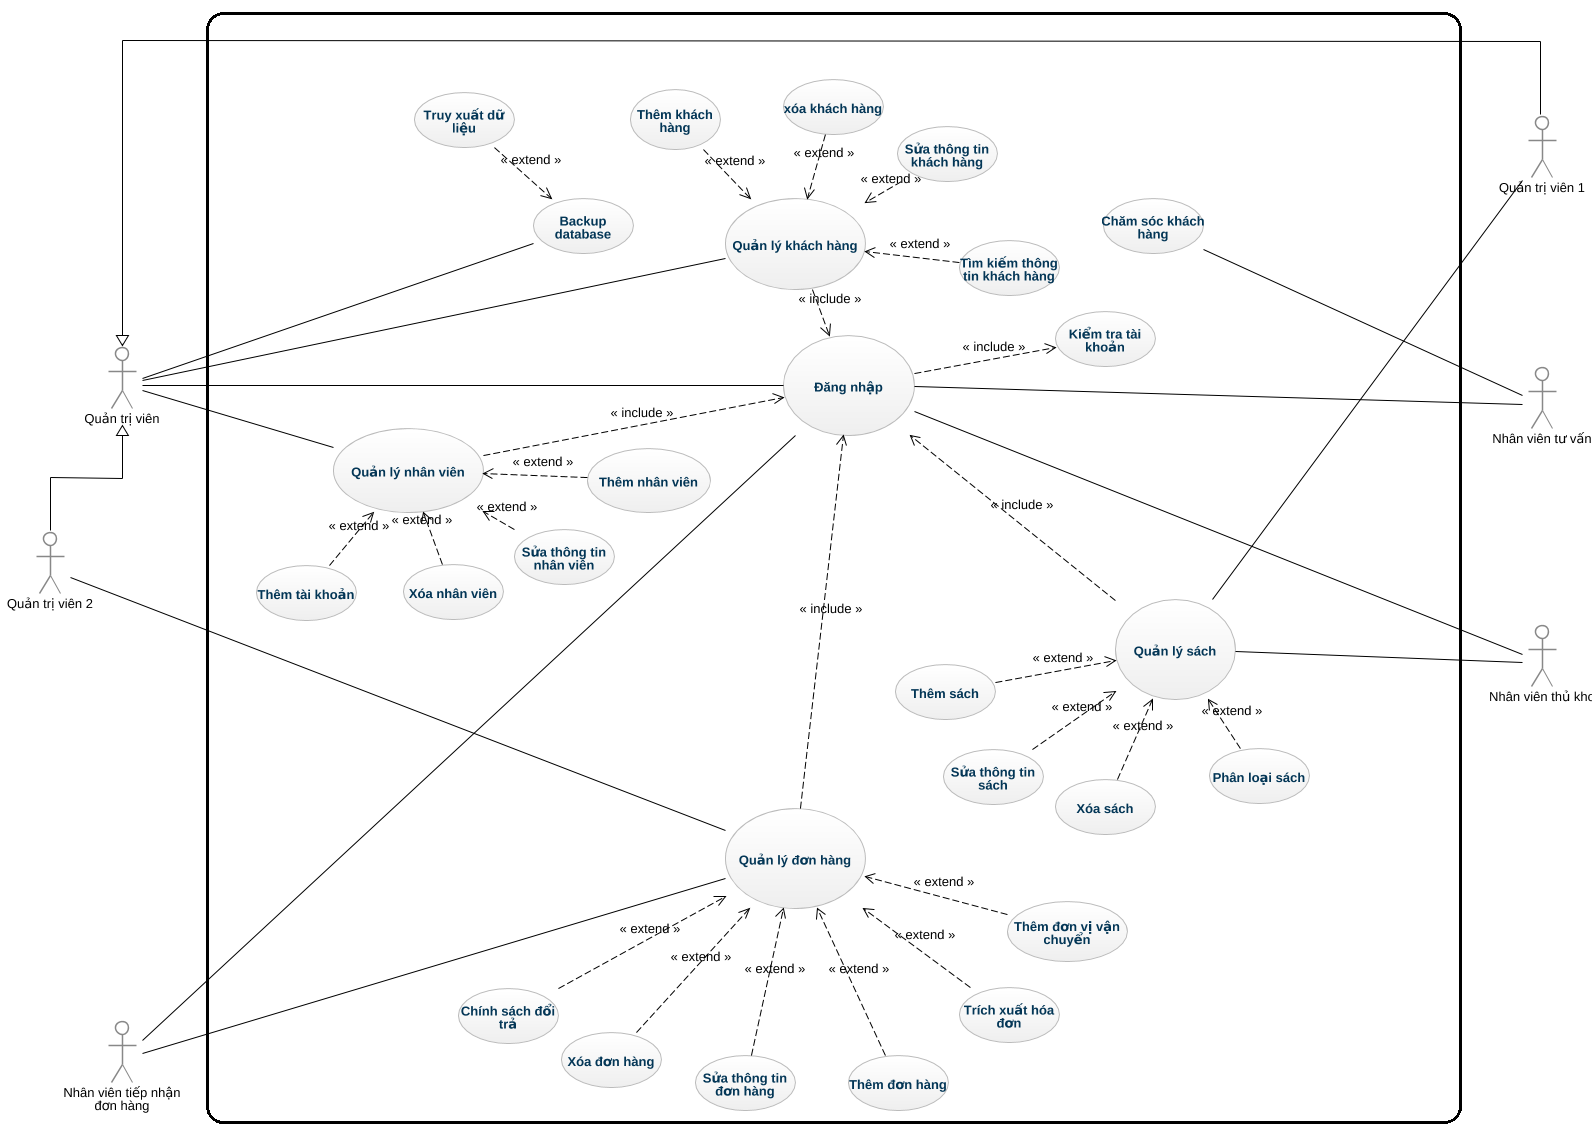
\includegraphics[scale = 0.3]{image/UseCaseDiagram_employee.png}
    \caption{Sơ đồ Use Case của các nhân viên và quản trị viên}
\end{figure}

\begin{figure}[htp]
    \centering
    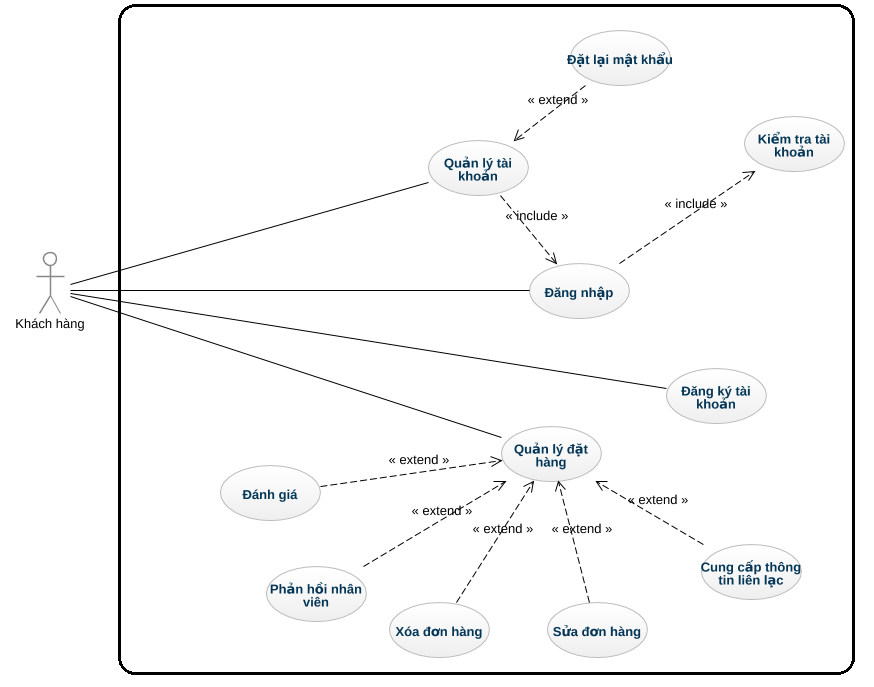
\includegraphics[scale = 0.5]{image/UseCaseDiagram_Customer.png}
    \caption{Sơ đồ Use Case của khách hàng}
\end{figure}


%------------------------------------------------------------------------------------------
%                                    Đặc tả Use Case
%------------------------------------------------------------------------------------------
\section{Đặc tả Use Case}
\subsection{\textit{Đặc tả use case Đăng nhập}}
\begin{figure}[htp]
    \centering
    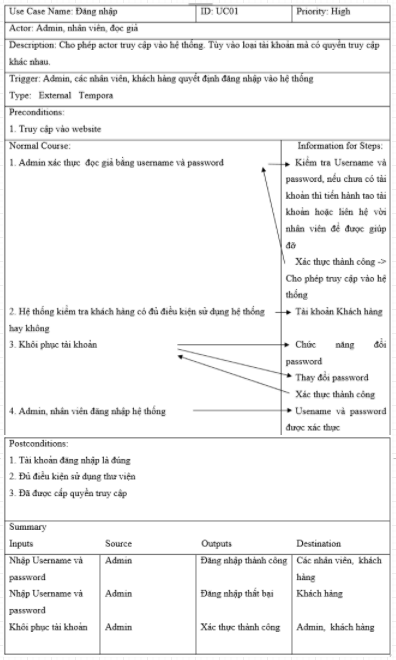
\includegraphics[scale = 0.94]{image/UC01.PNG}
    \caption{Đặc tả use case Đăng Nhập}
\end{figure}

\begin{figure}[htp]
    \subsection{\textit{Đặc tả use case Quản lý khách hàng}}
    \centering
    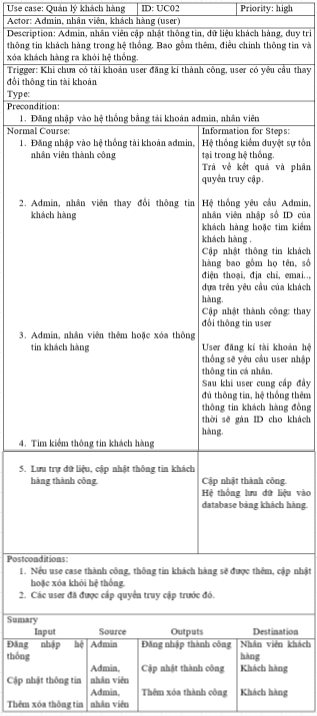
\includegraphics[scale = 1.2]{image/UC02.PNG}
    \caption{Đặc tả use case Quản lý khách hàng}
\end{figure}

\begin{figure}[htp]
    \subsection{\textit{Đặc tả use case Quản lý nhân viên}}
    \centering
    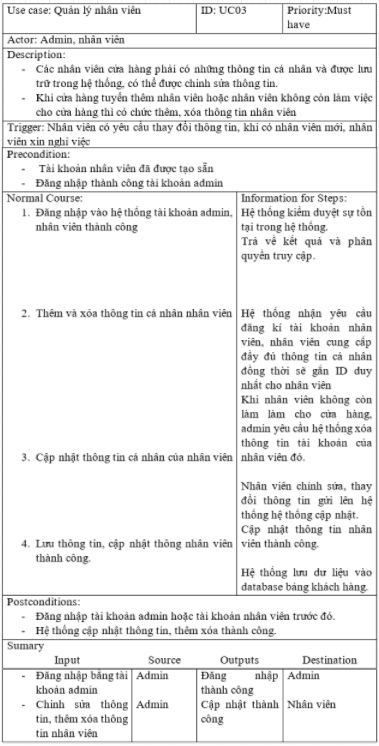
\includegraphics[scale = 1.15]{image/UC03.PNG}
    \caption{Đặc tả use case Quản lý nhân viên}
\end{figure}

%----------------------------------------------------------------------------------------
\pagebreak
%----------------------------------------------------------------------------------------

\begin{figure}[htp]
    \subsection{\textit{Đặc tả use case Quản lý sách}}
    \centering
    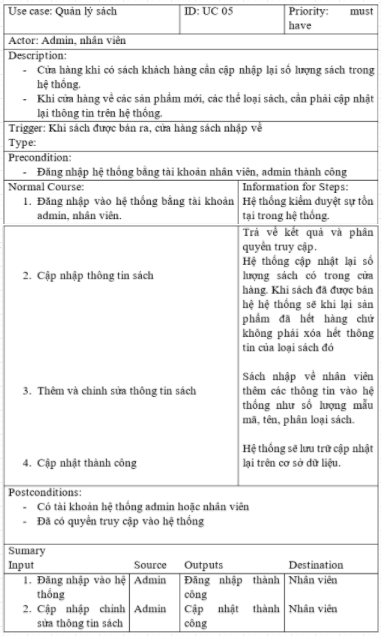
\includegraphics[scale = 1.34]{image/UC05.PNG}
    \caption{Đặc tả use case Quản lý sách}
\end{figure}

%----------------------------------------------------------------------------------------
\pagebreak
%----------------------------------------------------------------------------------------

\begin{figure}[htp]
    \subsection{\textit{Đặc tả use case Quản lý đơn hàng}}
    \centering
    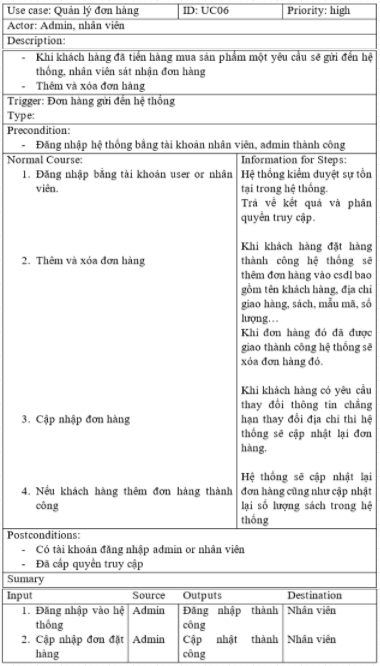
\includegraphics[scale = 1.3]{image/UC06.PNG}
    \caption{Đặc tả use case Quản lý đơn hàng}
\end{figure}

%----------------------------------------------------------------------------------------
\pagebreak
%----------------------------------------------------------------------------------------

\begin{figure}[htp]
    \subsection{\textit{Đặc tả use case Chăm sóc khách hàng}}
    \centering
    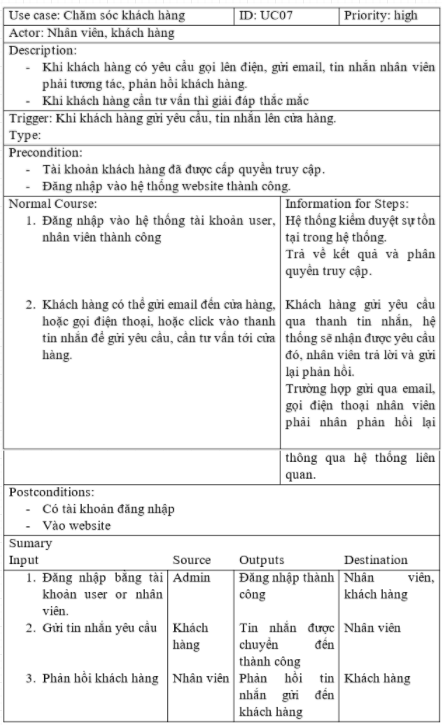
\includegraphics[scale = 1.2]{image/UC07.PNG}
    \caption{Đặc tả use case Chăm sóc khách hàng}
\end{figure}


%----------------------------------------------------------------------------------------
\pagebreak
%----------------------------------------------------------------------------------------

\begin{figure}[htp]
    \subsection{\textit{Đặc tả use case Quản lý đặt hàng}}
    \centering
    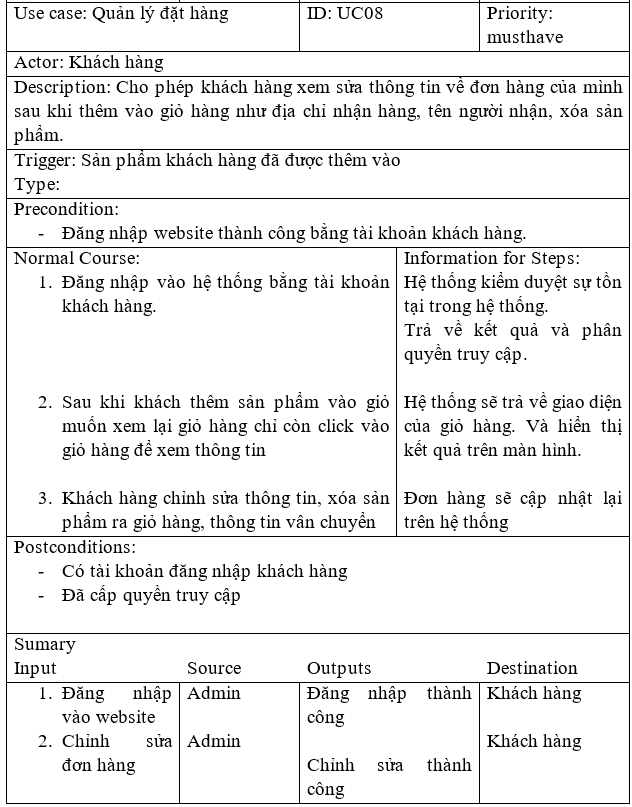
\includegraphics[scale = 1]{image/UC08.PNG}
    \caption{Đặc tả use case Quản lý đặt hàng}
\end{figure}

\begin{center}
    \begin{figure}[htp]
        \subsection{Đặc tả use case Quản lý tài khoản}
        \begin{center}
            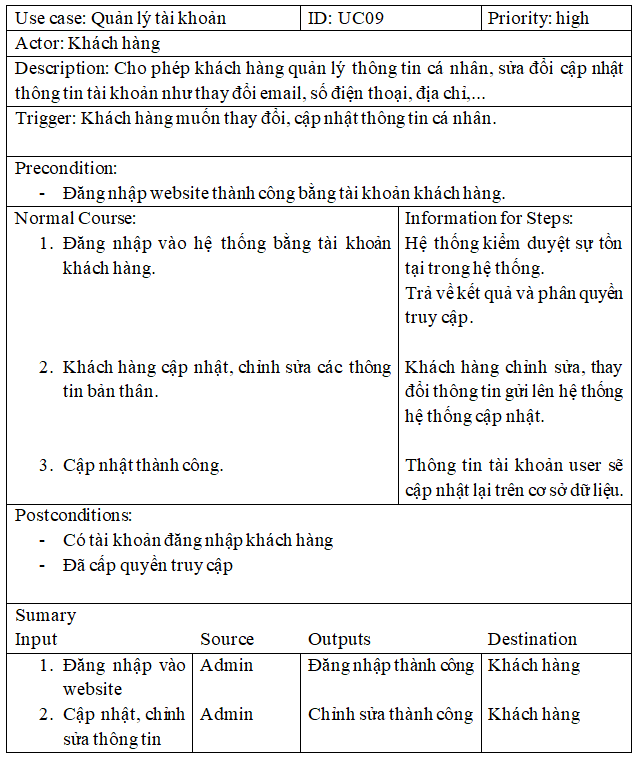
\includegraphics[scale = 1]{image/UC09.PNG}
        \end{center}
        \caption{Đặc tả use case Quản lý tài khoản}
        \label{refhinh1}
    \end{figure}
\end{center}

\begin{center}
    \begin{figure}[htp]
        \subsection{Đặc tả use case Đăng ký tài khoản}
        \begin{center}
            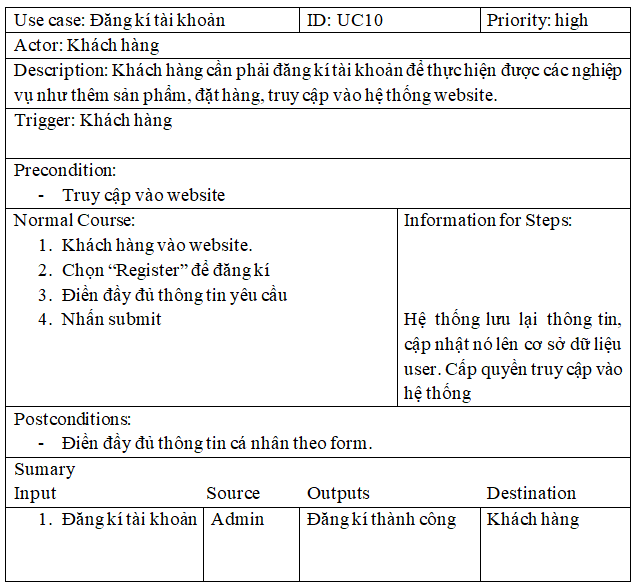
\includegraphics[scale = 1]{image/UC10.PNG}
        \end{center}
        \caption{Đặc tả use case Đăng ký tài khoản}
        \label{refhinh1}
    \end{figure}
\end{center}
%----------------------------------------------------------------------------------------
\pagebreak
%----------------------------------------------------------------------------------------

%------------------------------------------------------------------------------------------
%                                 Data Flow Diagram level content
%------------------------------------------------------------------------------------------
\begin{figure}[htp]
    \section{Sơ đồ DFD}
    \subsection{\textit{DFD level content}}
    \centering
    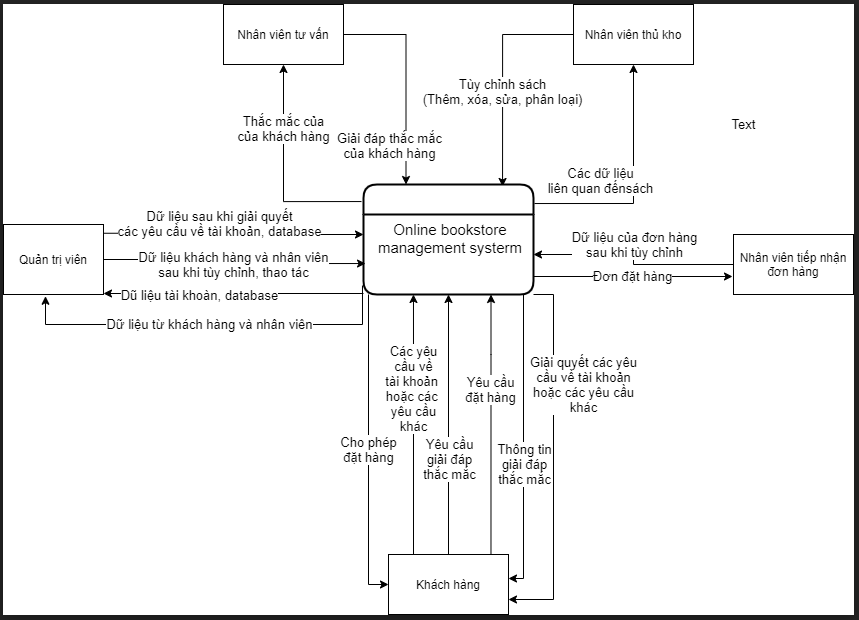
\includegraphics[scale = 0.8]{image/content.PNG}
    \caption{DFD level content}
\end{figure}

%------------------------------------------------------------------------------------------
%                                Data Flow Diagram level 1
%------------------------------------------------------------------------------------------
\begin{figure}[htp]
    \subsection{\textit{DFD level 1}}
    \centering
    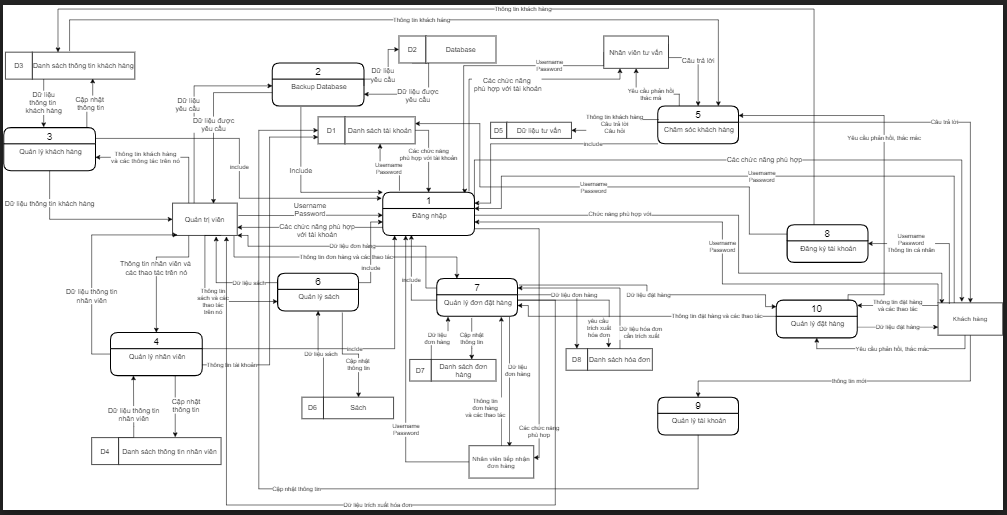
\includegraphics[scale = 0.6]{image/DFD_level1.PNG}
    \caption{DFD level 1}
\end{figure}


%------------------------------------------------------------------------------------------
%                               Data Flow Diagram level 2
%------------------------------------------------------------------------------------------
\begin{figure}[htp]
    \subsection{\textit{DFD level 2 của use case đăng nhập}}
    \centering
    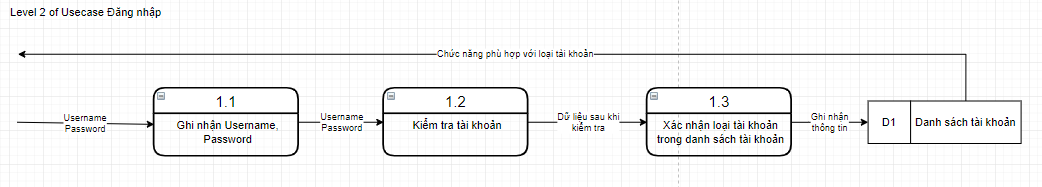
\includegraphics[scale = 0.6]{image/DFD_level2_dangnhap.PNG}
    \caption{DFD level 2 của use case Đăng nhập}
\end{figure}

\begin{figure}[htp]
    \subsection{\textit{DFD level 2 của use case backup database}}
    \centering
    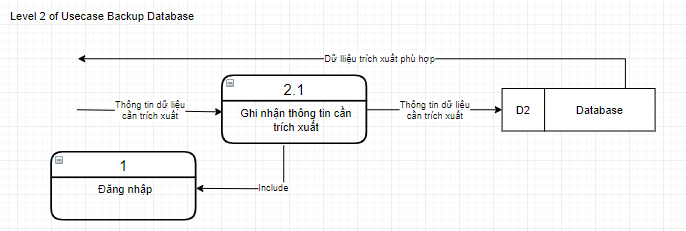
\includegraphics[scale = 0.8]{image/DFD_level2_backupDB.PNG}
    \caption{DFD level 2 của use case Backup Database}
\end{figure}

\begin{figure}[htp]
    \subsection{\textit{DFD level 2 của use case Quản lý khách hàng}}
    \centering
    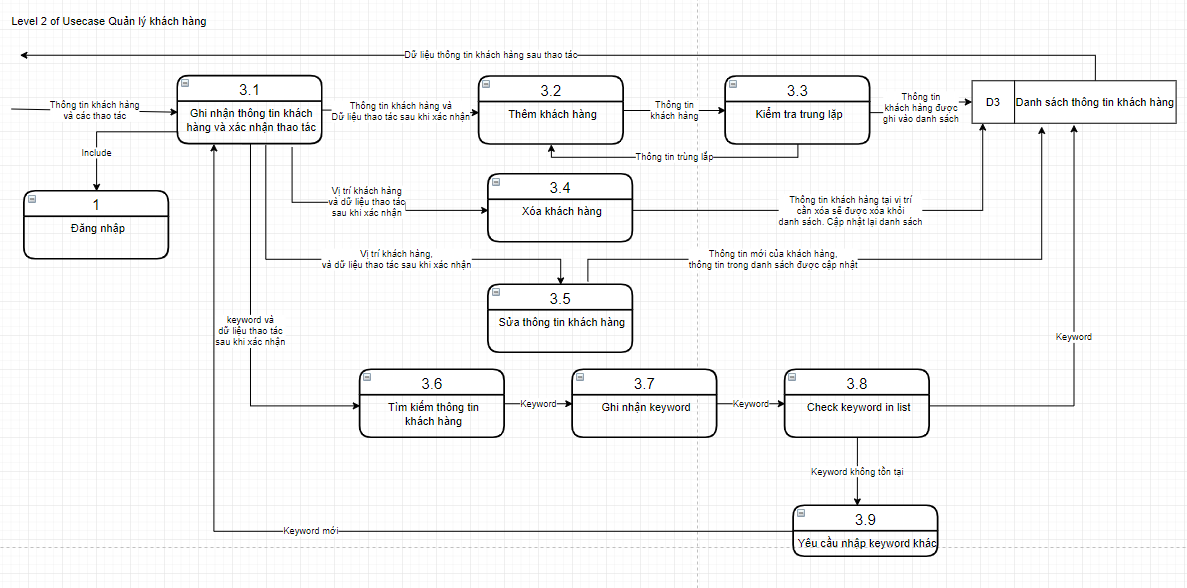
\includegraphics[scale = 0.55]{image/DFD_level2_qlkh.PNG}
    \caption{DFD level 2 của use case Quản lý khách hàng}
\end{figure}

\begin{figure}[htp]
    \subsection{\textit{DFD level 2 của use case Quản lý nhân viên}}
    \centering
    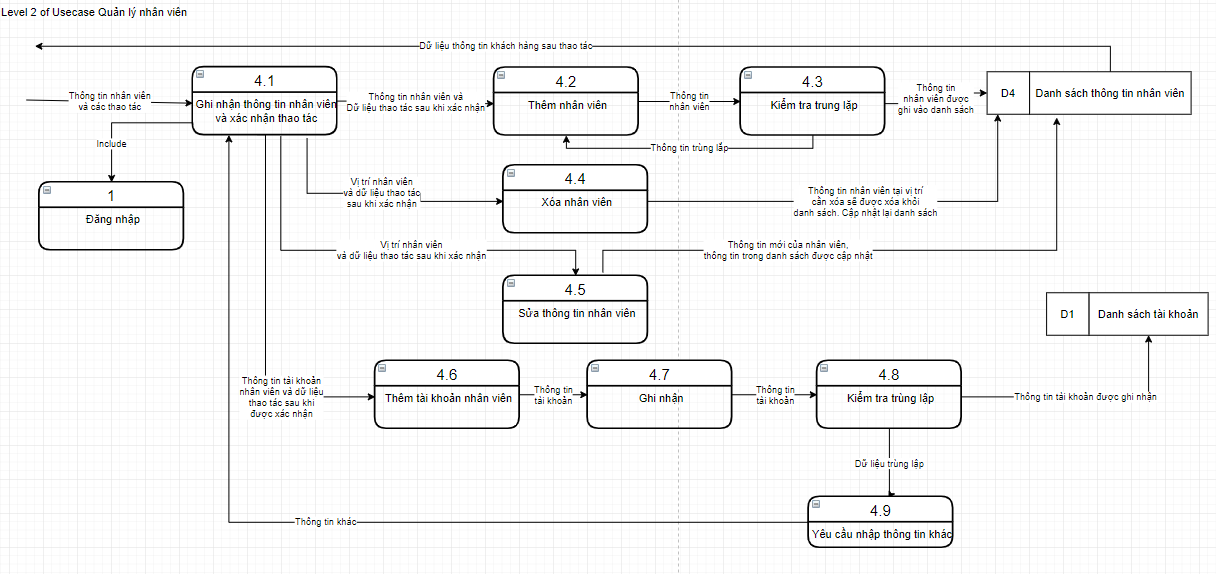
\includegraphics[scale = 0.5]{image/DFD_level2_qlnv.PNG}
    \caption{DFD level 2 của use case Quản lý nhân viên}
\end{figure}

\begin{figure}[htp]
    \subsection{\textit{DFD level 2 của use case Chăm sóc khách hàng}}
    \centering
    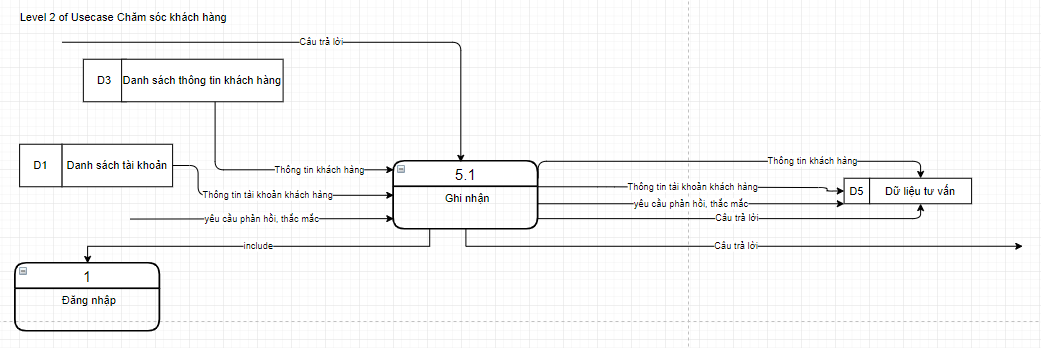
\includegraphics[scale = 0.6]{image/DFD_level2_cskh.PNG}
    \caption{DFD level 2 của use case Chăm sóc khách hàng}
\end{figure}

\begin{figure}[htp]
    \subsection{\textit{DFD level 2 của use case Quản lý sách}}
    \centering
    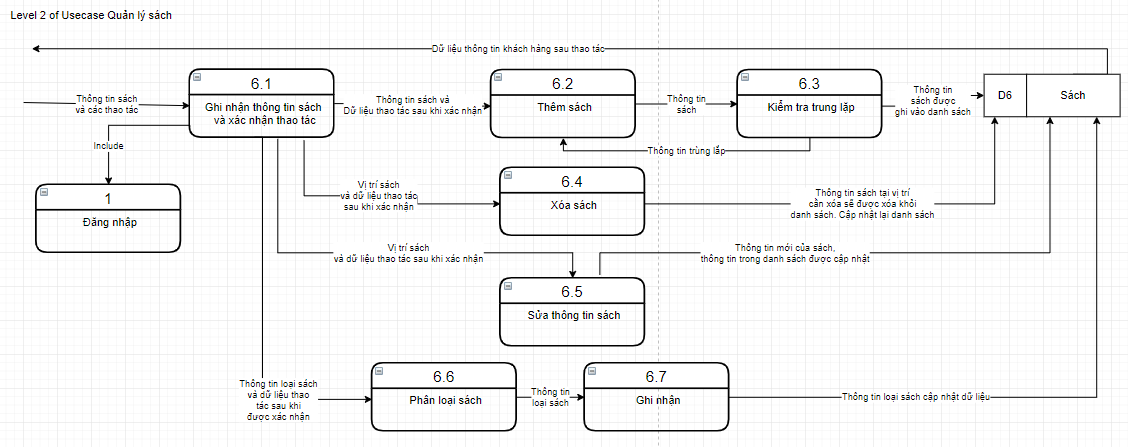
\includegraphics[scale = 0.6]{image/DFD_level2_qls.PNG}
    \caption{DFD level 2 của use case Quản lý sách}
\end{figure}

\begin{figure}[htp]
    \subsection{\textit{DFD level 2 của use case Quản lý đơn hàng}}
    \centering
    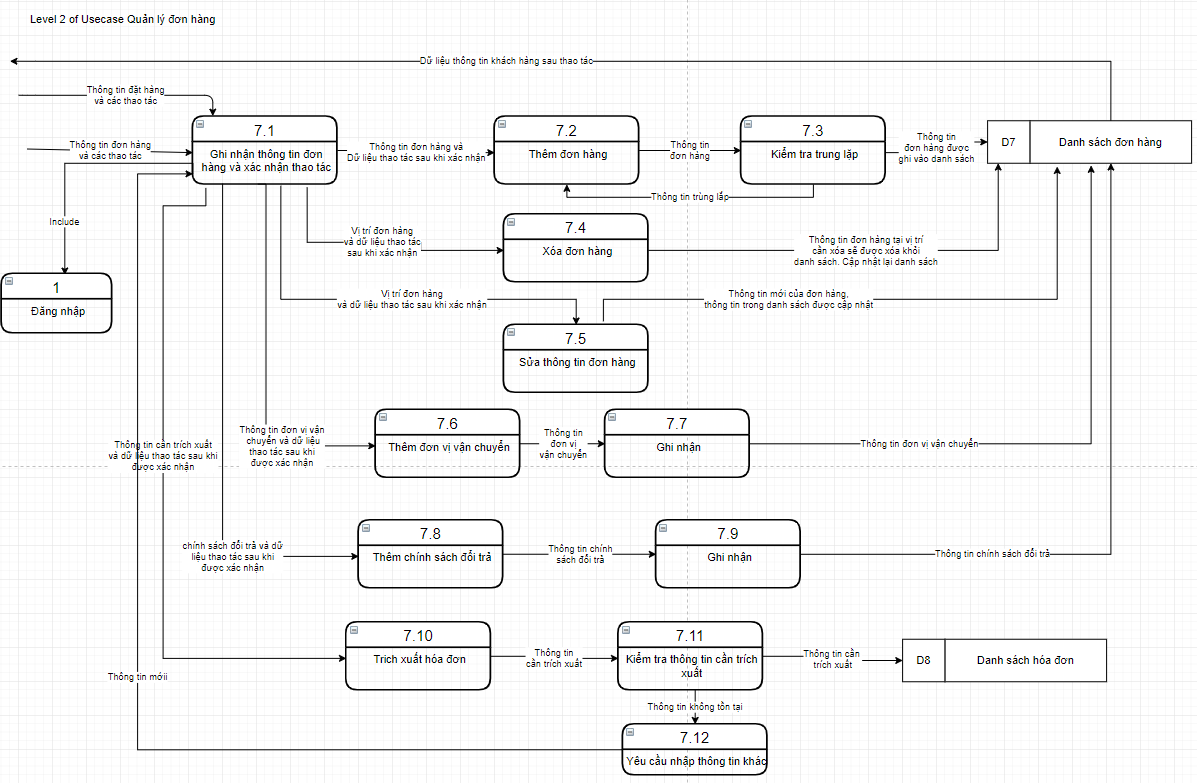
\includegraphics[scale = 0.6]{image/DFD_level2_qldh.PNG}
    \caption{DFD level 2 của use case Quản lý đơn hàng}
\end{figure}

\begin{figure}[htp]
    \subsection{\textit{DFD level 2 của use case Đăng ký tài khoản}}
    \centering
    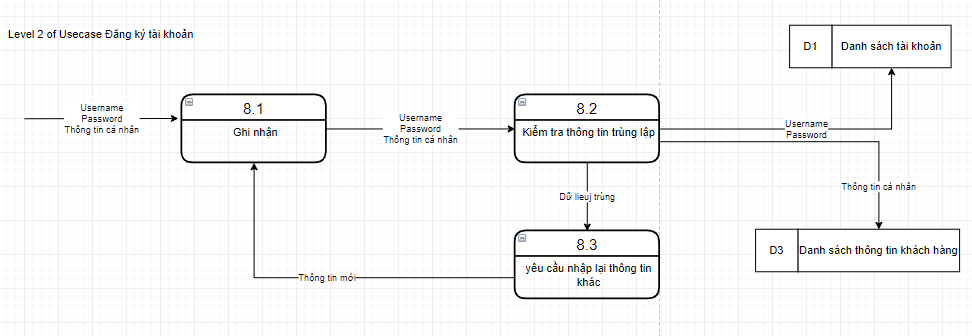
\includegraphics[scale = 0.6]{image/DFD_level2_dktk.PNG}
    \caption{DFD level 2 của use case Đăng ký tài khoản}
\end{figure}

\begin{figure}[htp]
    \subsection{\textit{DFD level 2 của use case Quản lý tài khoản}}
    \centering
    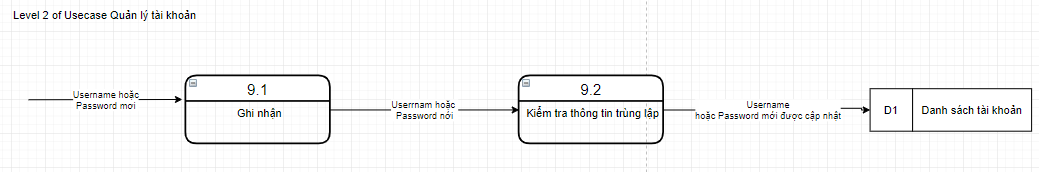
\includegraphics[scale = 0.6]{image/DFD_level2_qltk.PNG}
    \caption{DFD level 2 của use case Quản lý tài khoản}
\end{figure}

\begin{figure}[htp]
    \subsection{\textit{DFD level 2 của use case Quản lý đặt hàng}}
    \centering
    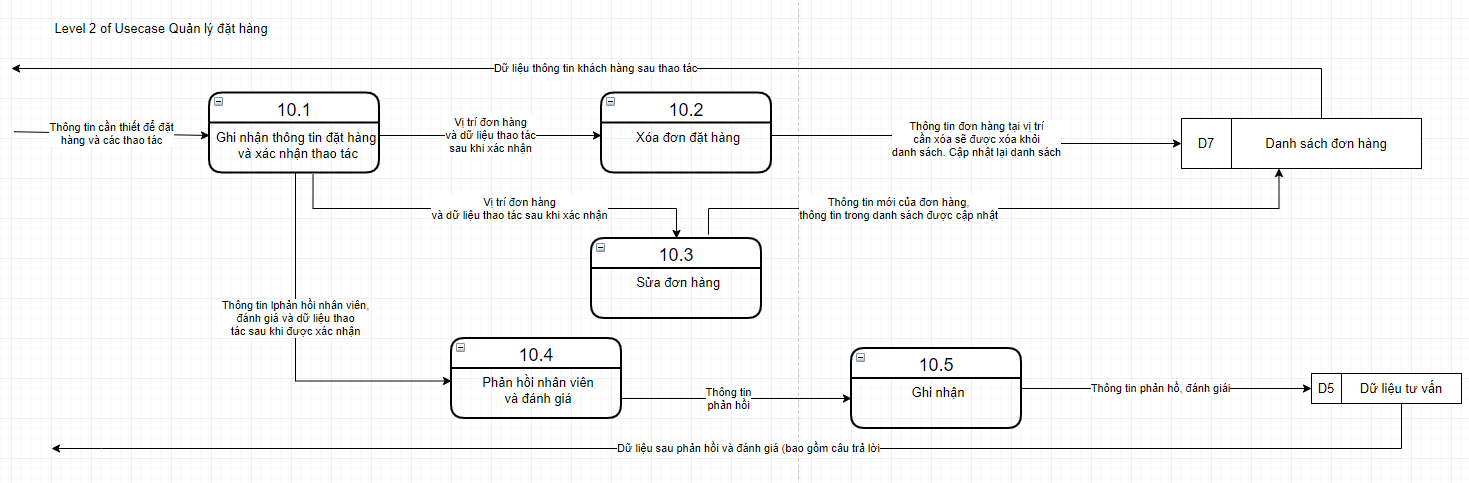
\includegraphics[scale = 0.45]{image/DFD_level2_qldathang.PNG}
    \caption{DFD level 2 của use case Quản lý đặt hàng}
\end{figure}


%------------------------------------------------------------------------------------------
%                                    Activity Diagram
%------------------------------------------------------------------------------------------
\begin{figure}[htp]
    \section{Activity Diagram}
    \subsection{\textit{Activity diagram của use case Đăng nhập}}
    \centering
    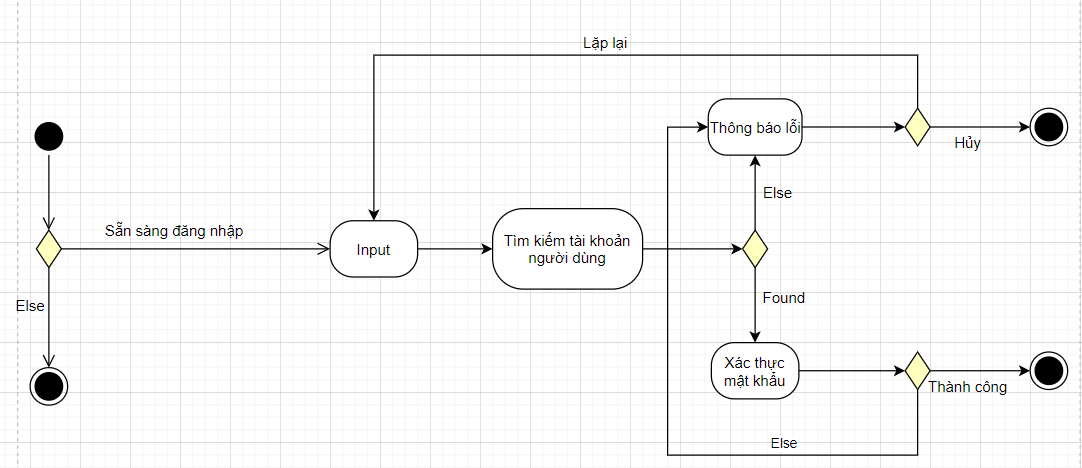
\includegraphics[scale = 0.6]{image/activity_dangnhap.PNG}
    \caption{Activity diagram của use case Đăng nhập}
\end{figure}

\begin{figure}[htp]
    \subsection{\textit{Activity diagram của use case Quản lý khách hàng}}
    \centering
    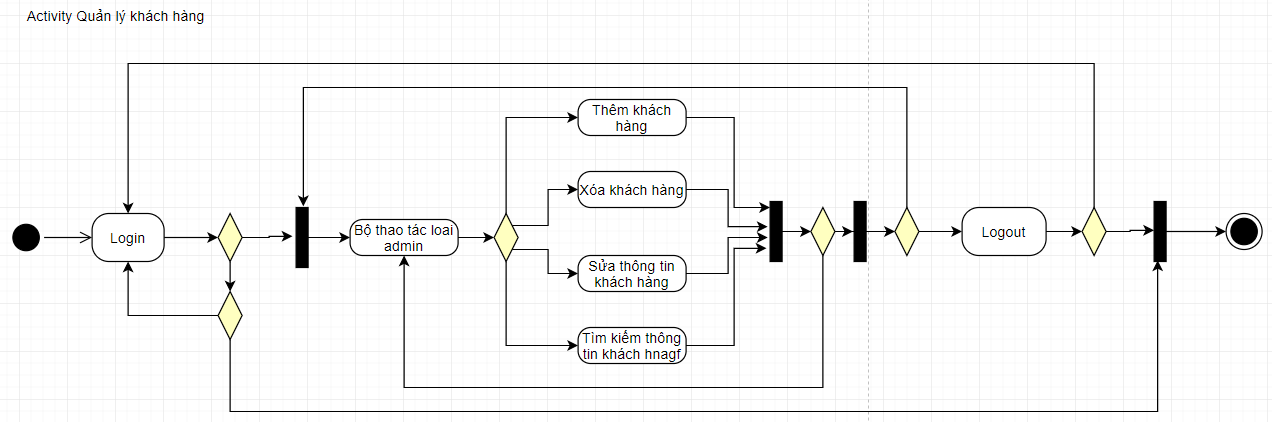
\includegraphics[scale = 0.55]{image/activity_qlkh.PNG}
    \caption{Activity diagram của use case Quản lý khách hàng}
\end{figure}

\begin{figure}[htp]
    \subsection{\textit{Activity diagram của use case Backup Database}}
    \centering
    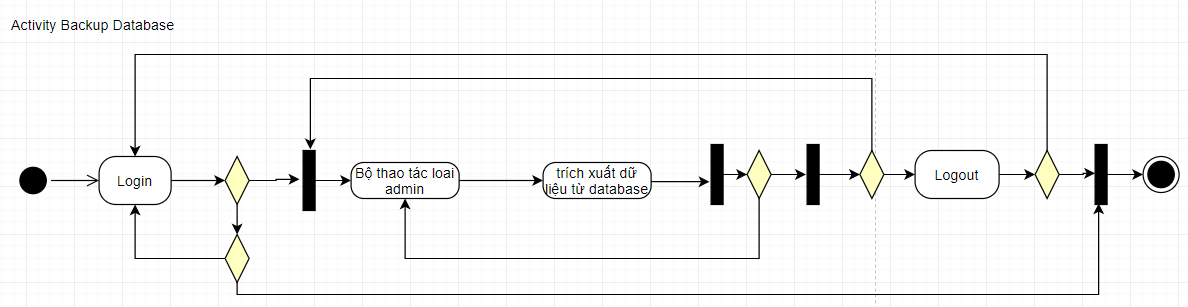
\includegraphics[scale = 0.6]{image/activity_backupDB.PNG}
    \caption{Activity diagram của use case Backup Database}
\end{figure}

\begin{figure}[htp]
    \subsection{\textit{Activity diagram của use case Quản lý nhân viên}}
    \centering
    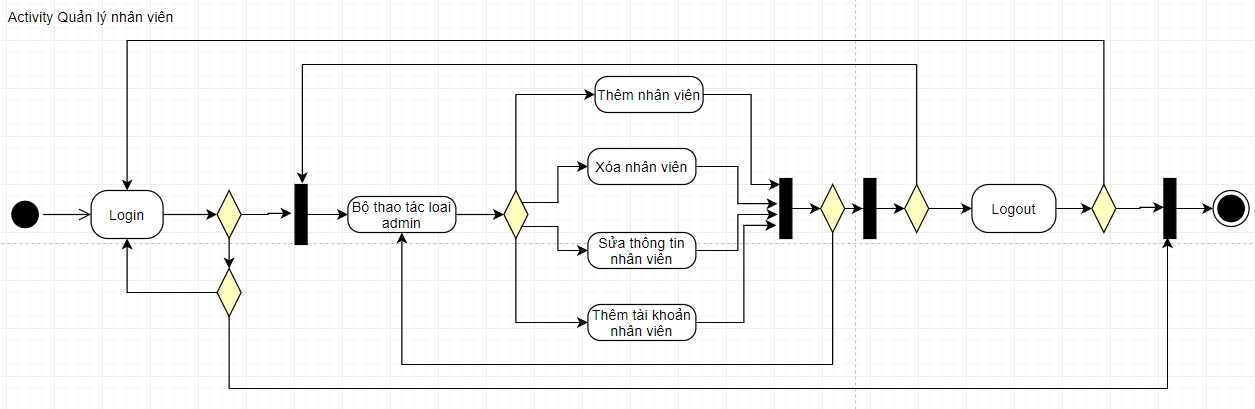
\includegraphics[scale = 0.55]{image/activity_qlnv.PNG}
    \caption{Activity diagram của use case Quản lý nhân viên}
\end{figure}

\begin{figure}[htp]
    \subsection{\textit{Activity diagram của use case Chăm sóc khách hàng}}
    \centering
    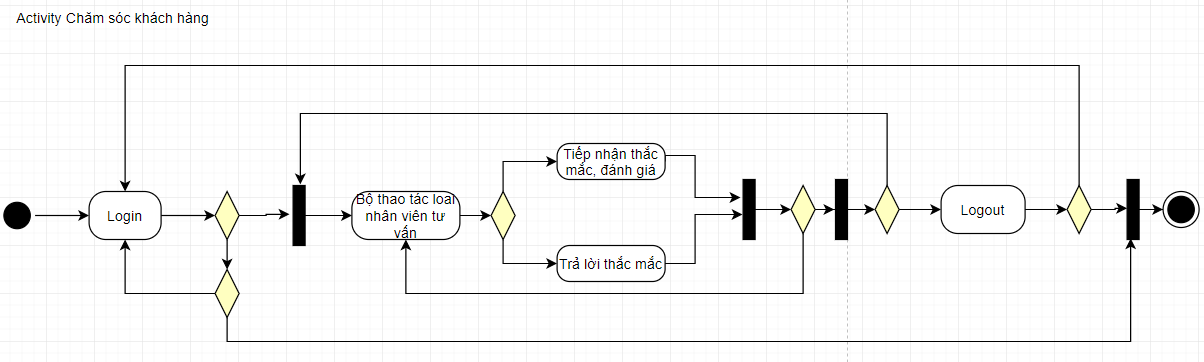
\includegraphics[scale = 0.55]{image/activity_cskh.PNG}
    \caption{Activity diagram của use case Chăm sóc khách hàng}
\end{figure}

\begin{figure}[htp]
    \subsection{\textit{Activity diagram của use case Quản lý sách}}
    \centering
    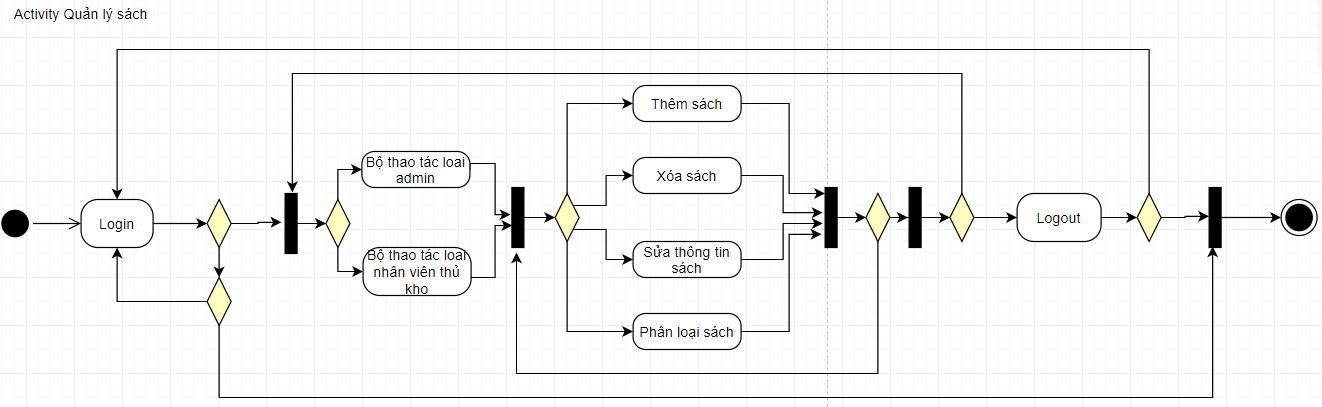
\includegraphics[scale = 0.5]{image/activity_qls.PNG}
    \caption{Activity diagram của use case Quản lý sách}
\end{figure}

\begin{figure}[htp]
    \subsection{\textit{Activity diagram của use case Quản lý đơn hàng}}
    \centering
    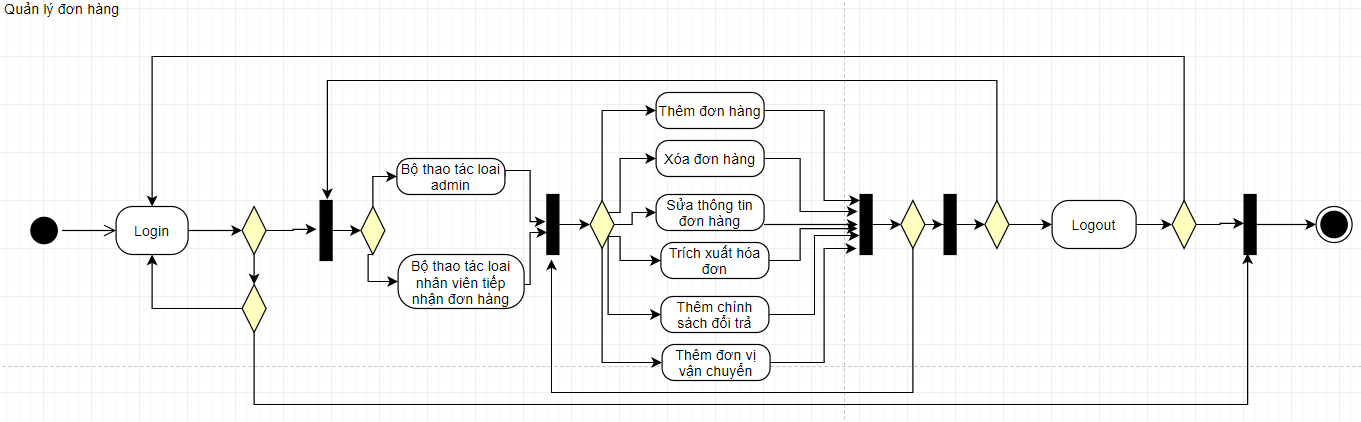
\includegraphics[scale = 0.5]{image/activity_qldh.PNG}
    \caption{Activity diagram của use case Quản lý đơn hàng}
\end{figure}

\begin{figure}[htp]
    \subsection{\textit{Activity diagram của use case Đăng ký tài khoản}}
    \centering
    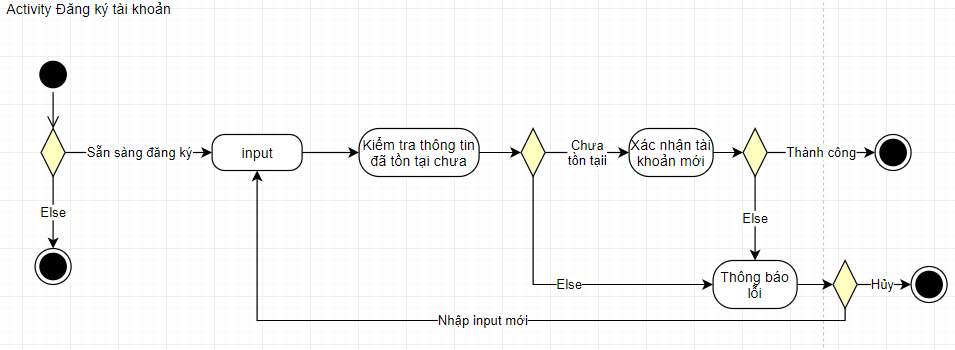
\includegraphics[scale = 0.6]{image/activity_dktk.PNG}
    \caption{Activity diagram của use case Đăng ký tài khoản}
\end{figure}

\begin{figure}[htp]
    \subsection{\textit{Activity diagram của use case Quản lý tài khoản}}
    \centering
    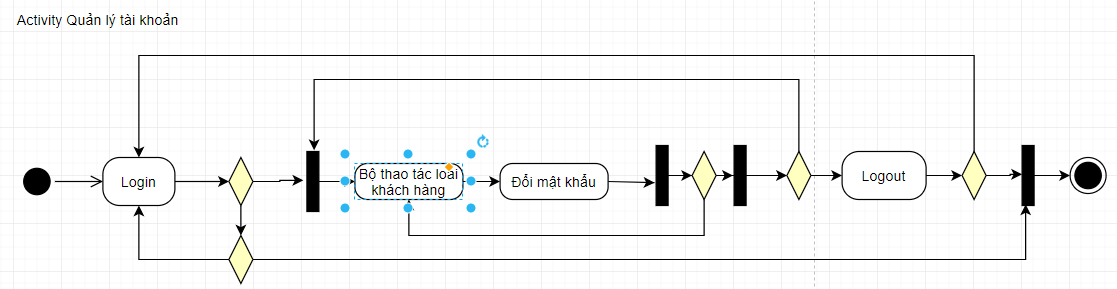
\includegraphics[scale = 0.55]{image/activity_qltk.PNG}
    \caption{Activity diagram của use case Quản lý tài khoản}
\end{figure}

\begin{figure}[htp]
    \subsection{\textit{Activity diagram của use case Quản lý đặt hàng}}
    \centering
    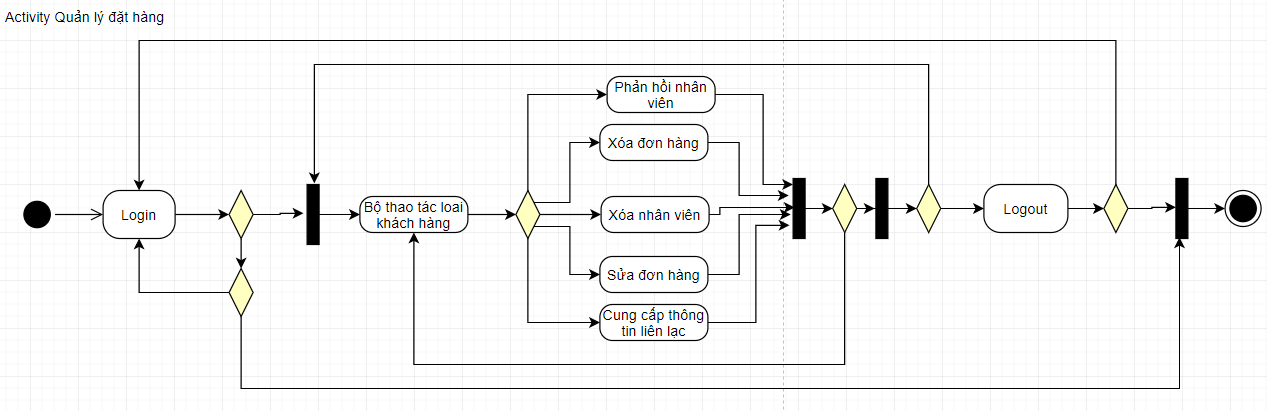
\includegraphics[scale = 0.5]{image/activity_qldathang.PNG}
    \caption{Activity diagram của use case Quản lý đặt hàng}
\end{figure}

%----------------------------------------------------------------------------------------
\pagebreak
%----------------------------------------------------------------------------------------

%------------------------------------------------------------------------------------------
%                                    Sequence Diagram
%------------------------------------------------------------------------------------------
\begin{center}
    \begin{figure}[htp]
        \section{Sơ đồ tuần tự (Sequence Diagram}
        \subsection{Đăng nhập}
        \begin{center}
            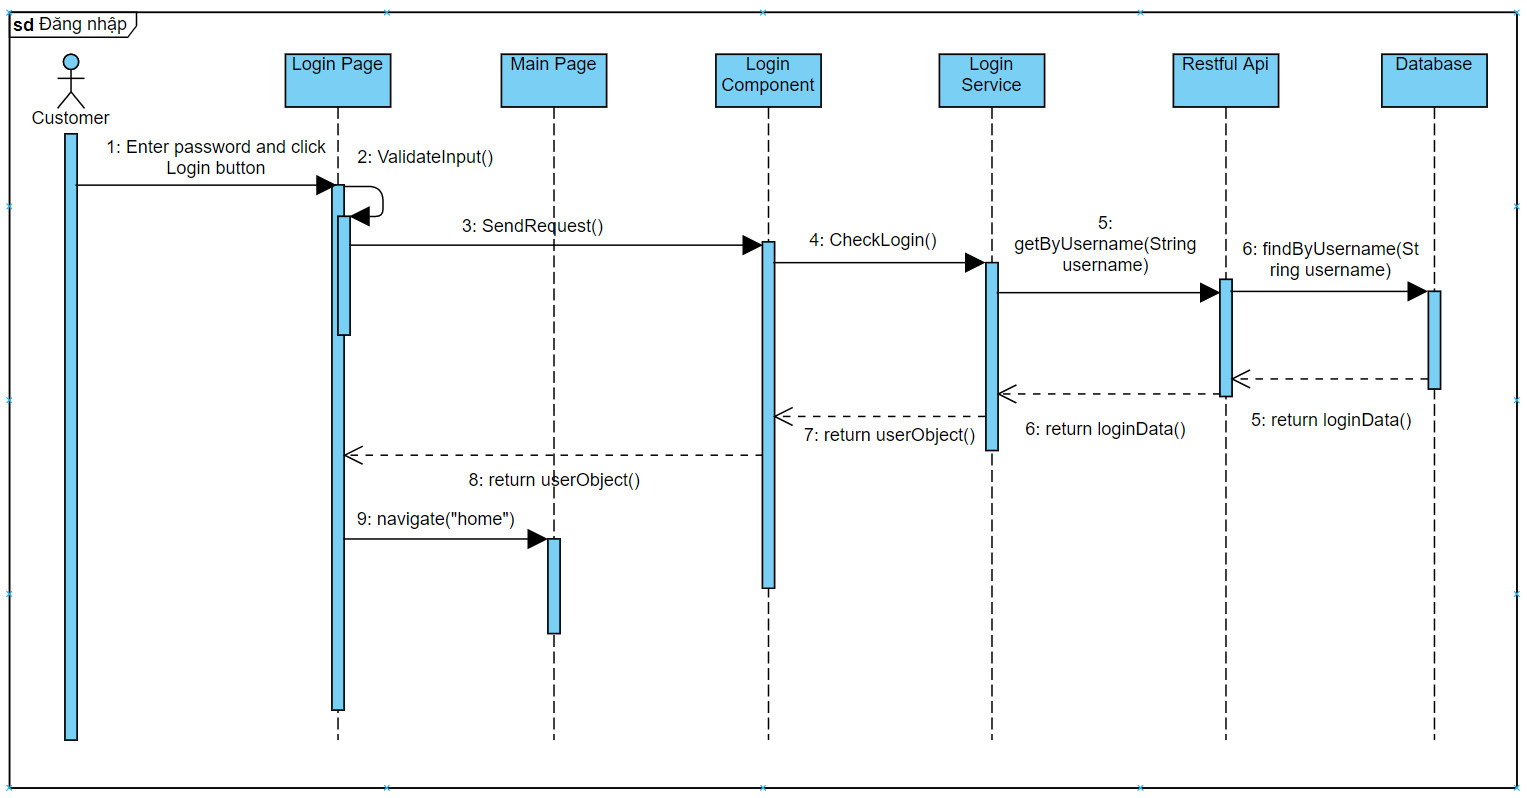
\includegraphics[scale = 0.5]{image/sequence_dangnhap.png}
        \end{center}
        \caption{Sequence Diagram Đăng nhập}
    \end{figure}
\end{center}

\begin{center}
    \begin{figure}[htp]
        \subsection{Thêm sách bán}
        \begin{center}
            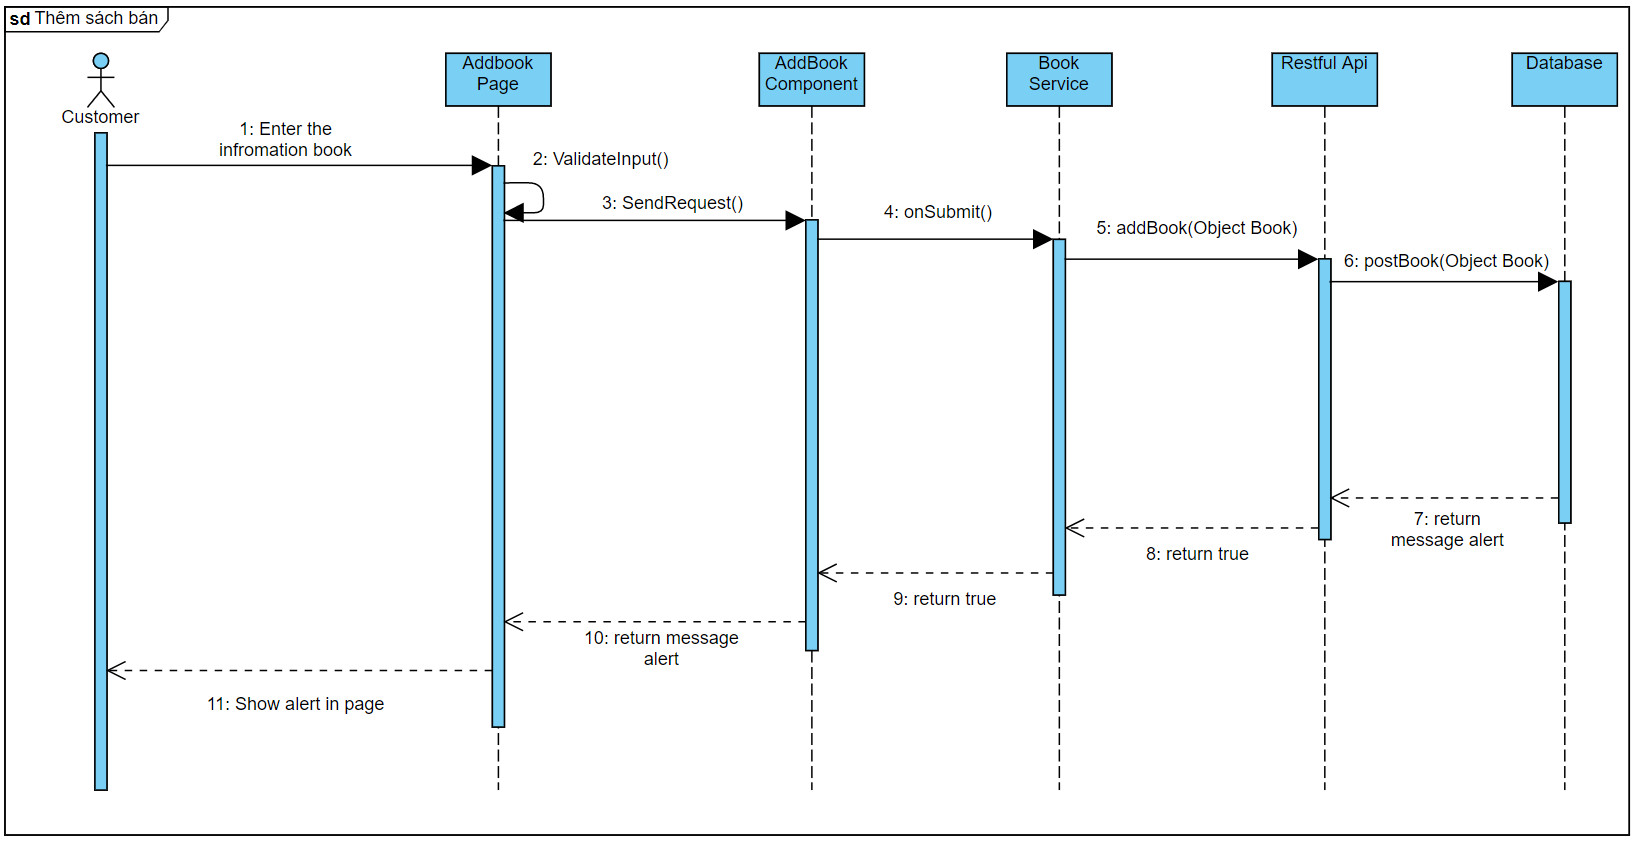
\includegraphics[scale = 0.5]{image/sequence_addBook.png}
        \end{center}
        \caption{Sequence Diagram Thêm sách bán}
    \end{figure}
\end{center}

%----------------------------------------------------------------------------------------
\pagebreak
%----------------------------------------------------------------------------------------

\begin{center}
    \begin{figure}[htp]
        \subsection{Thêm nhân viên}
        \begin{center}
            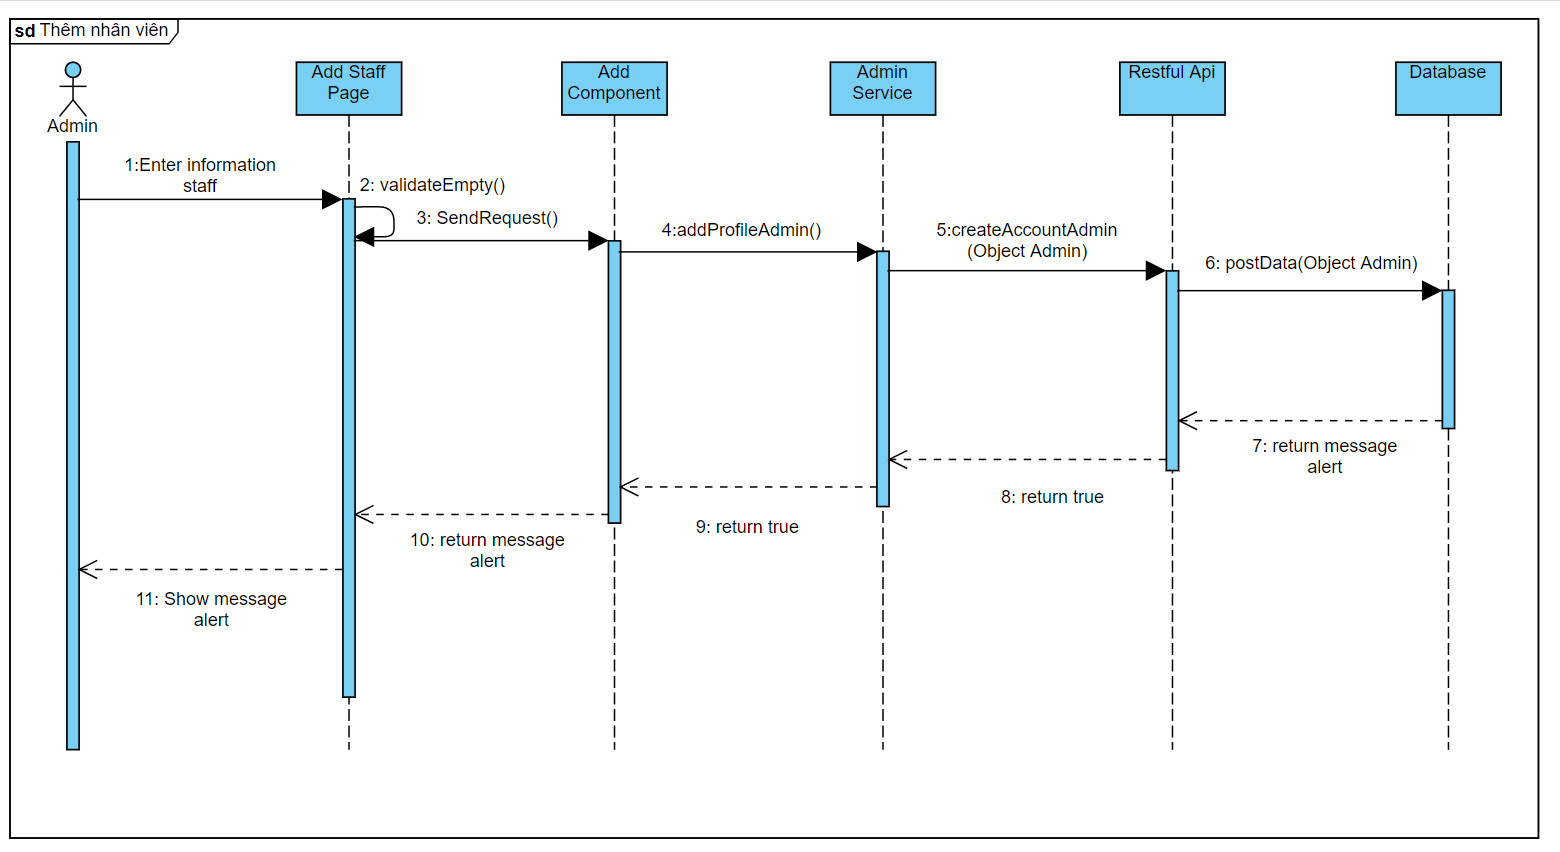
\includegraphics[scale = 0.5]{image/sequence_addemplyee.png}
        \end{center}
        \caption{Sequence Diagram Thêm nhân viên}
    \end{figure}
\end{center}

\begin{center}
    \begin{figure}[htp]
        \subsection{Kiểm soát lượt truy cập}
        \begin{center}
            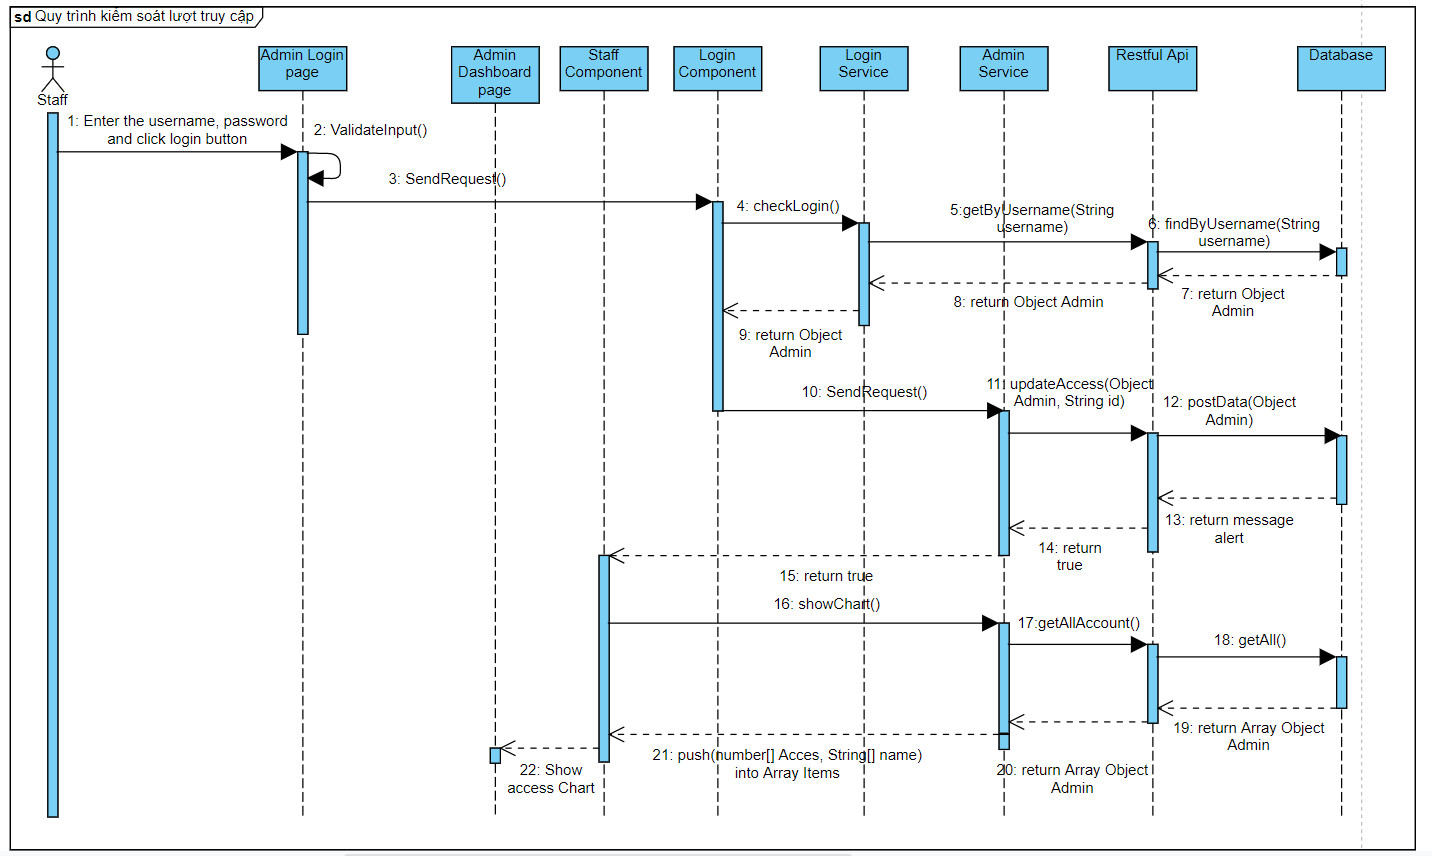
\includegraphics[scale = 0.5]{image/kiemsoatluottruycap.png}
        \end{center}
        \caption{Sequence Diagram Kiểm soát lượt truy cập}
    \end{figure}
\end{center}

%----------------------------------------------------------------------------------------
\pagebreak
%----------------------------------------------------------------------------------------

%------------------------------------------------------------------------------------------
%                               Information Flow Diagram
%------------------------------------------------------------------------------------------
\begin{center}
    \begin{figure}[htp]
        \section{Information Flow Diagram (IFD)}
        \subsection{Thêm sách}
        \begin{center}
            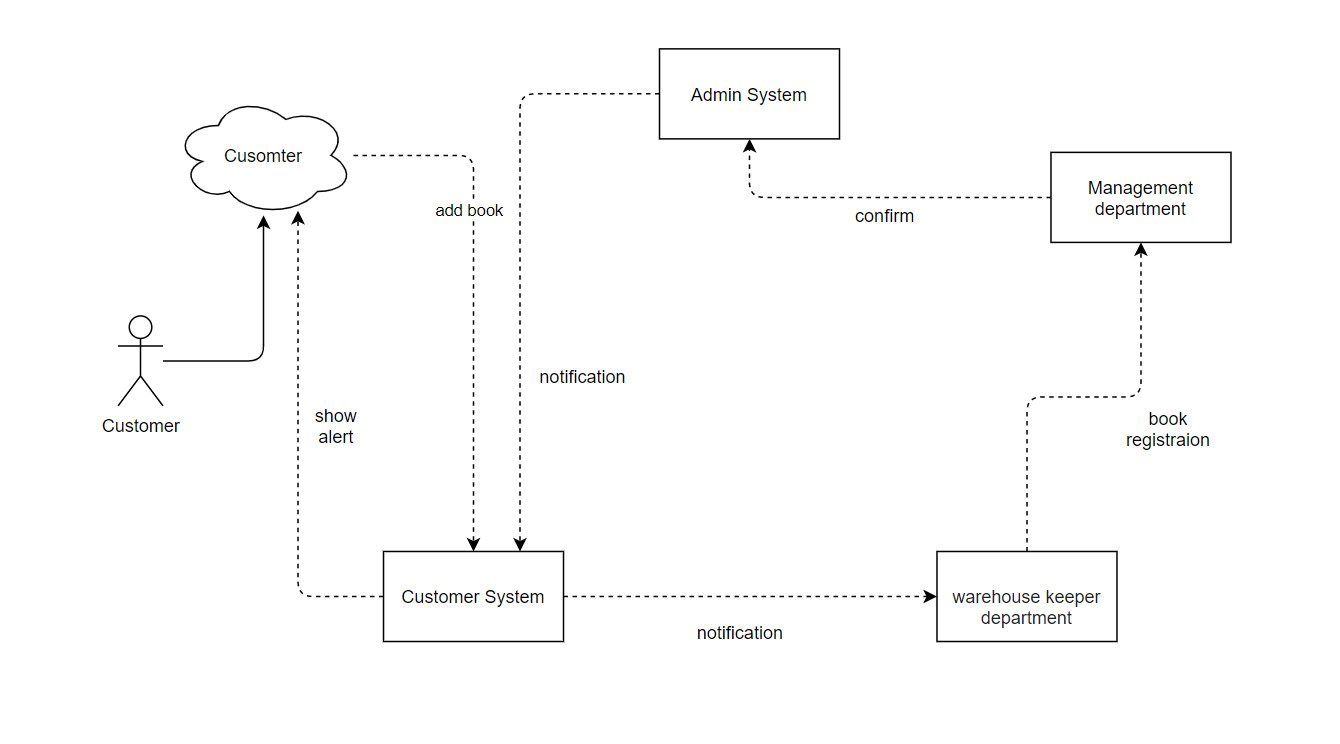
\includegraphics[scale = 0.65]{image/ifd_addbook.png}
        \end{center}
        \caption{Information Flow Diagram Thêm sách}
    \end{figure}
\end{center}

\begin{center}
    \begin{figure}[htp]
        \subsection{Quy trình bán hàng}
        \begin{center}
            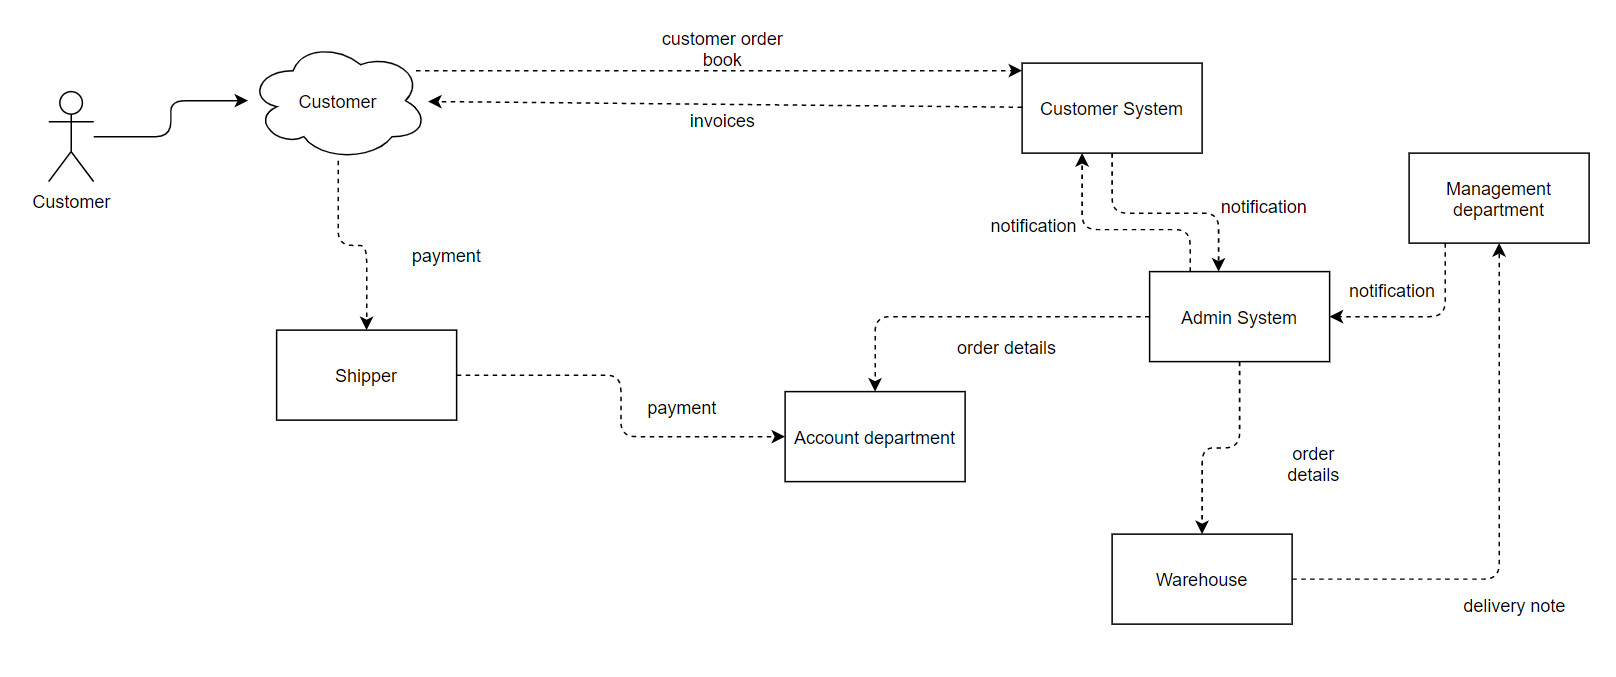
\includegraphics[scale = 0.5]{image/ifd_quytrinhbanhang.png}
        \end{center}
        \caption{Information Flow Diagram Quy trình bán hàng}
    \end{figure}
\end{center}

\begin{center}
    \begin{figure}[htp]
        \subsection{Thêm sách (admin - quản trị viên)}
        \begin{center}
            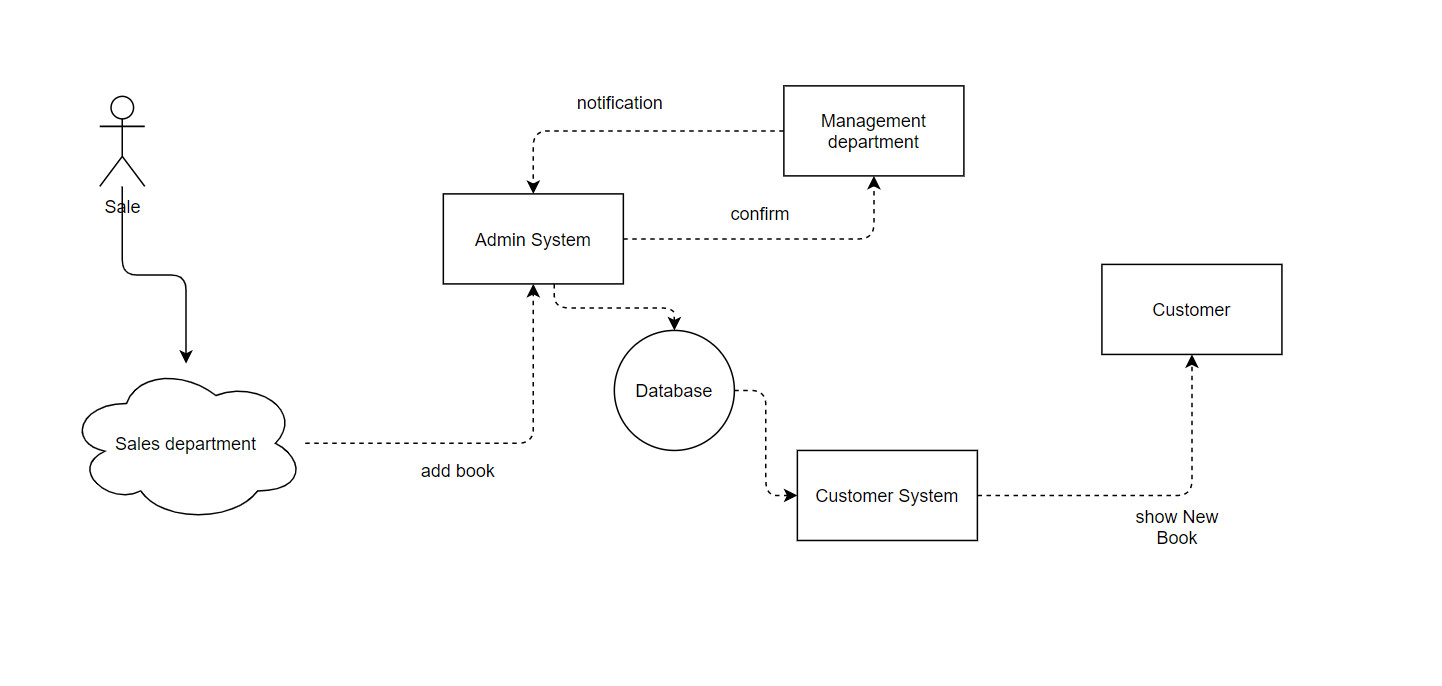
\includegraphics[scale = 0.65]{image/ifd_addbook_admin.png}
        \end{center}
        \caption{Information Flow Diagram Thêm sách (admin - quản trị viên)}
    \end{figure}
\end{center}

\begin{center}
    \begin{figure}[htp]
        \subsection{Gửi câu hỏi}
        \begin{center}
            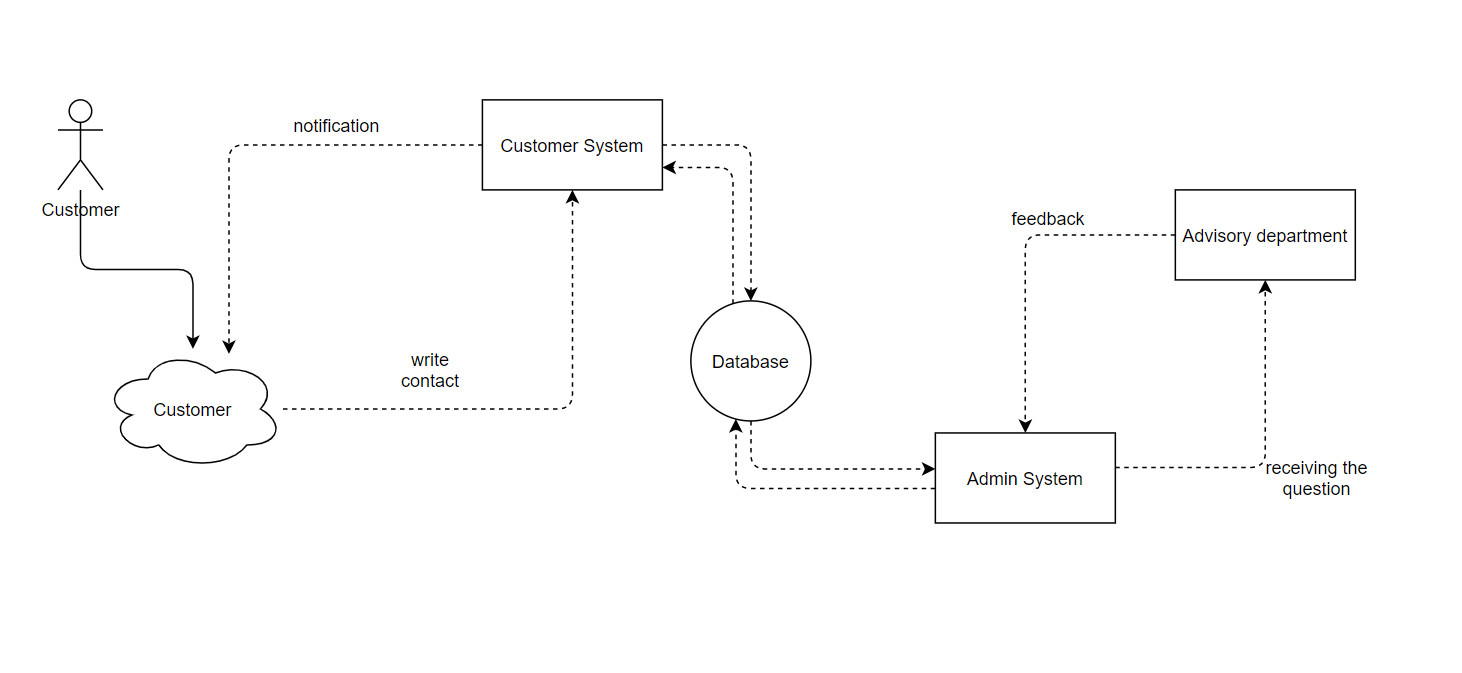
\includegraphics[scale = 0.55]{image/ifd_guicauhoi.png}
        \end{center}
        \caption{Information Flow Diagram Gửi câu hỏi}
    \end{figure}
\end{center}


%------------------------------------------------------------------------------------------
%                                    Class Diagram
%------------------------------------------------------------------------------------------
\begin{center}
    \begin{figure}[htp]
        \section{Sơ đồ lớp (Class Diagram)}
        \begin{center}
            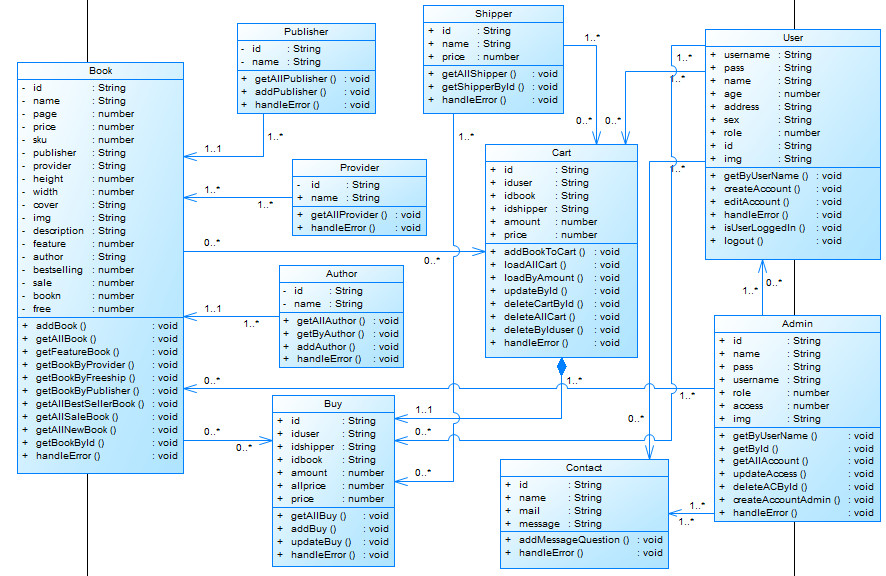
\includegraphics[scale = 0.7]{image/classdiagram.png}
        \end{center}
        \caption{Class Diagram}
    \end{figure}
\end{center}

%------------------------------------------------------------------------------------------
%                                   Mô hình thực thể ERD
%------------------------------------------------------------------------------------------
\begin{center}
    \begin{figure}[htp]
        \section{Mô hình thực thể ERD}
        \begin{center}
            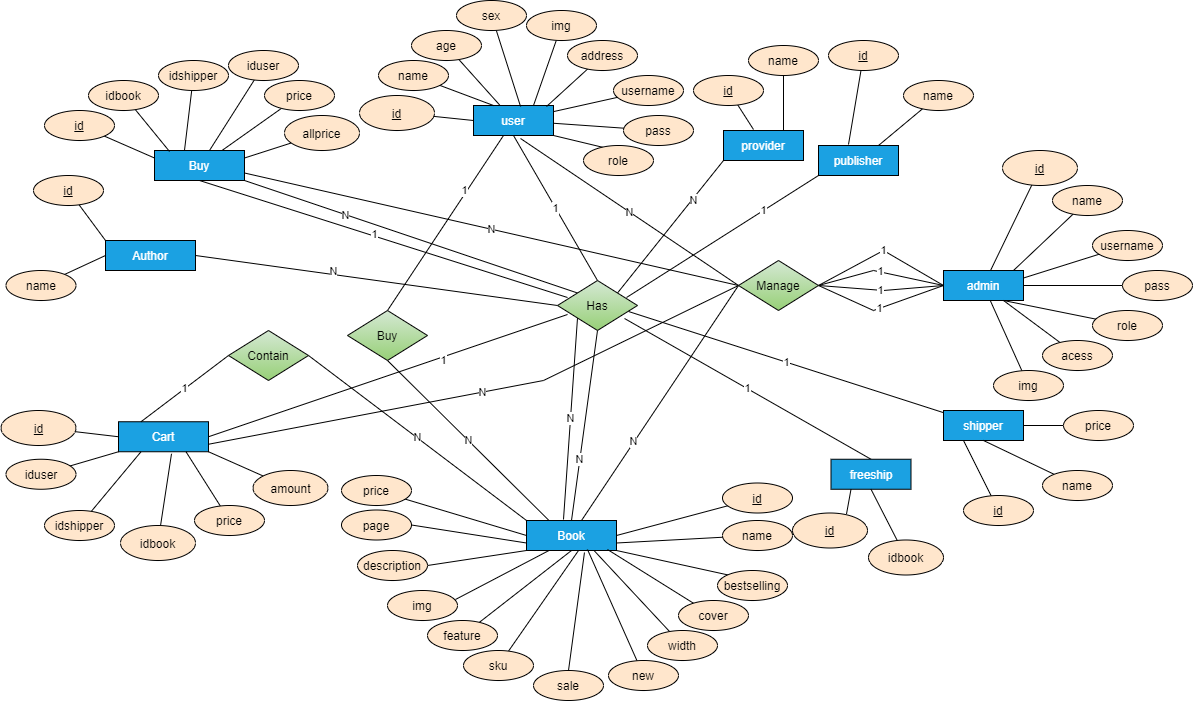
\includegraphics[scale = 0.44]{image/ERD.PNG}
        \end{center}
        \caption{Mô hình thực thể ERD(Entity Relationship Diagram)}
    \end{figure}
\end{center}

\end{document}